\documentclass[../Text/00main.tex]{subfiles}
\graphicspath{{../}}

\begin{document}

The results of this study will be sub-divided into seven smaller sections. First, the performance of the model will be evaluated on the basis of Goodness-of-Fit analysis in the validation section. Then the simulation results follow in four sections covering model complexity, strike, dip, and rake variation, depth variation and finally a small integration of results in a Mw 7.0 example scenario. Each of the sections will be followed by a discussion of results and their implications.

\section{Validation}\label{sec:validation}

\subsection{Large domain Çubuk}


\begin{figure}[htb!]
    \centering
    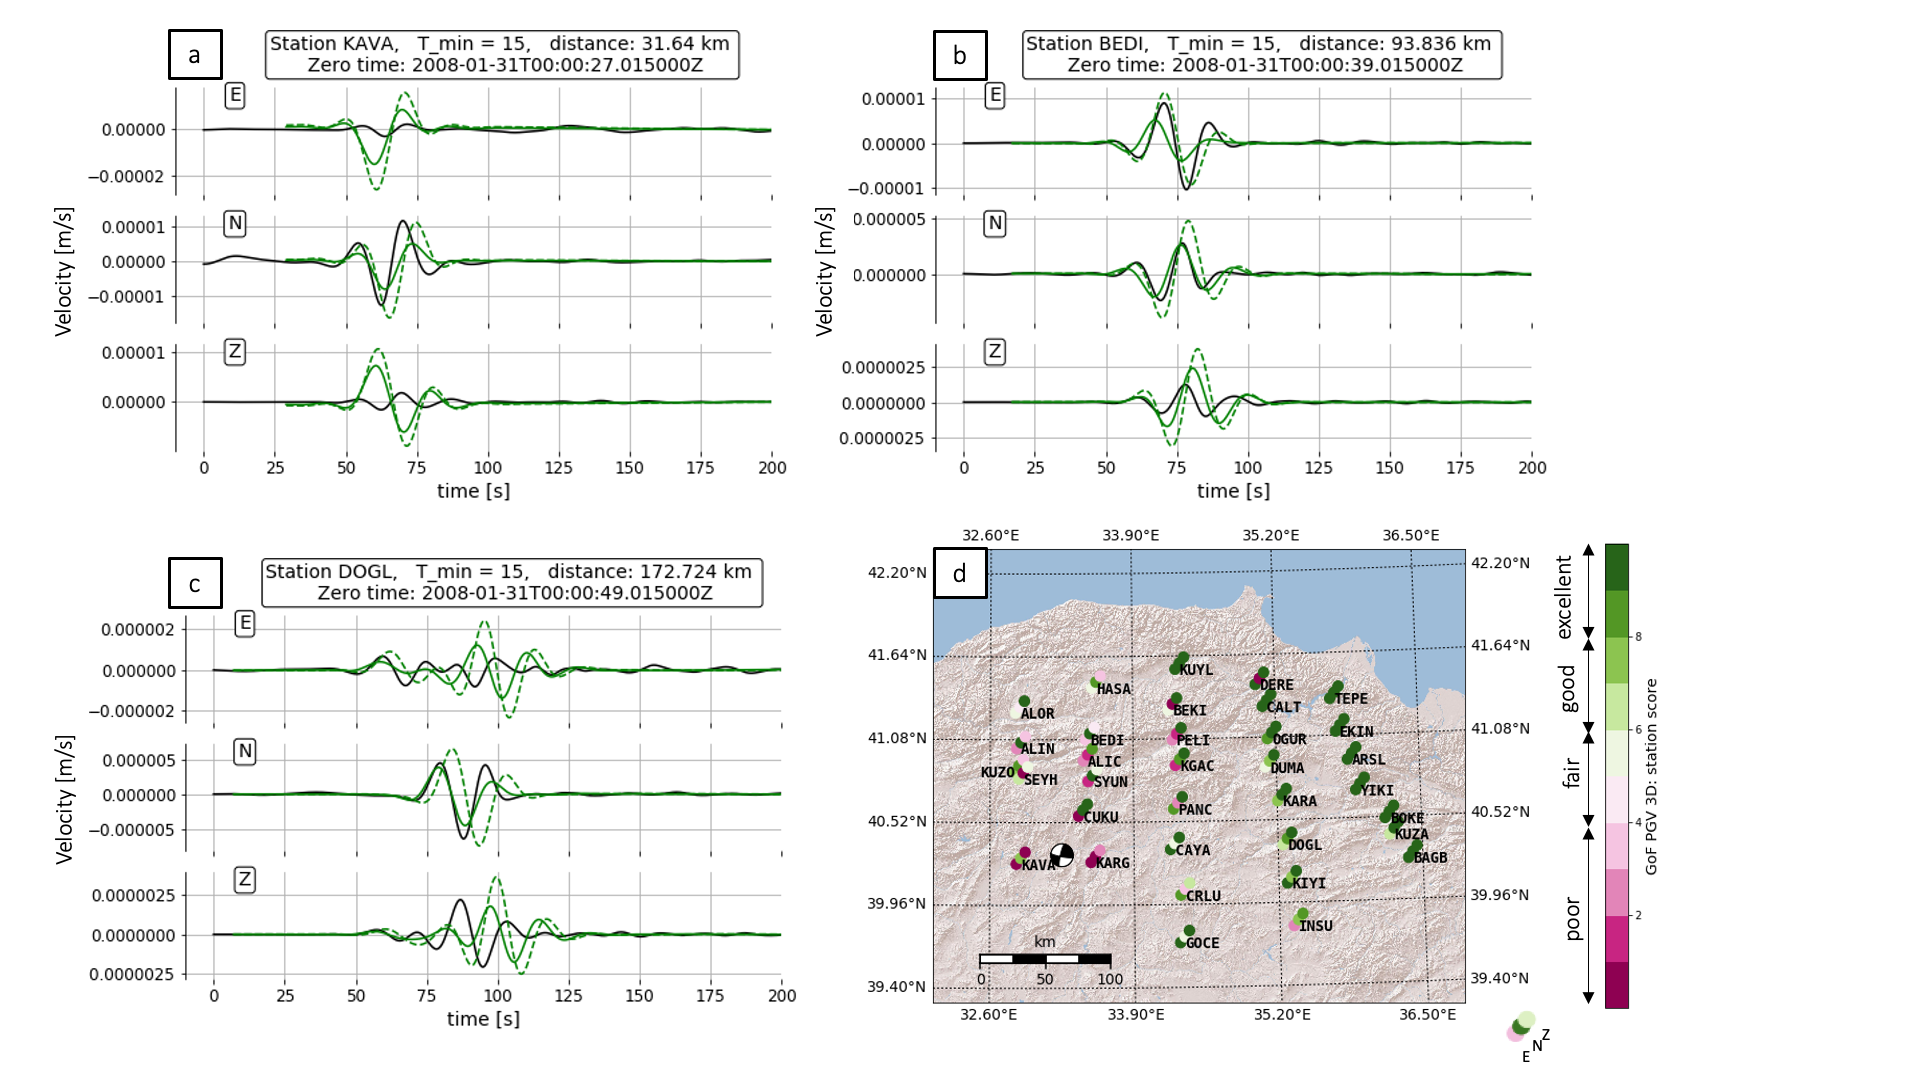
\includegraphics[width=1\linewidth]{images_results/waveforms_large.png}%
    \caption{Example of the comparison of 3D (green) and 1D (green, dashed) simulated velocity time series with the observed data (black). Station ALIN (a) and station TEPE (b). All signals are bandpass-filtered at 0.067 Hz.}%
    \label{fig:TEPEandALIN}%
\end{figure}



In this validation we compare the output of our forward model with measured data from the Mw 4.9 event described in Figure \ref{fig:cubukeventinfo}. Two examples of the 37 receivers are given in Figure \ref{fig:TEPEandALIN}.  More results at 15 Hz are given in Appendix \ref{app:validation}. Examination of the waveforms shows that the fit varies between receivers and E, N and Z components. For the 3D model, the amplitudes generally match well with the data, whereas the 1D model consistently over-estimates the maximum amplitude at this frequency. The start-time of the main waveform, and the duration of the signal after the main waveform is generally not reproduced accordingly by the simulation.

\begin{figure}
    \centering
    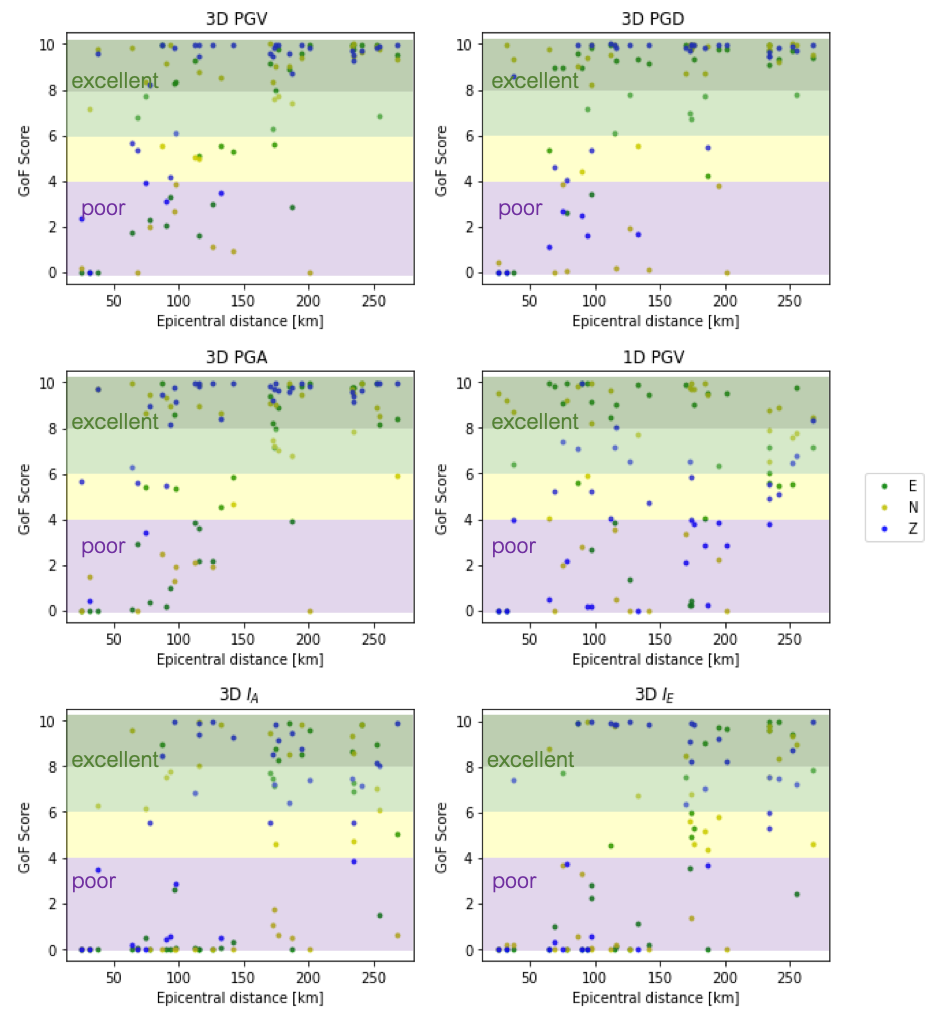
\includegraphics[width=.7\linewidth]{images_results/gofepicentral.png}
    \caption{Results of the large-domain PGA, PGV, PGD for the 3D model and PGV for the 1D model, as well as Arias intensity and the Energy integral. All data in E, N and Z direction with respect to epicentral distance.}
    \label{fig:gofpot_epicentral_large}
\end{figure}

 Apart from visual comparison, we employ the GoF measures discussed in Section \ref{ssec:GoF_explain}. The spectral parameters are not evaluated for the large domain, as the low frequency only covers the first frequency band suggested for analysis by \citet{anderson_quantitative_nodate}. Figure \ref{fig:gofpot_epicentral_large} shows that the fit of the intensity measures is improving with epicentral distance for the peak-based parameters using a 3D model. This trend is especially strong with the Z-component. The 1D model shows a less clear improvement with epicentral distance. %iets over teleseismic distances??
 % move this?

% If you use beamer only pass "xcolor=table" option, i.e. 
%\documentclass[xcolor=table]{beamer}
\begin{table}[h!]
\caption{Table of the a selection of \cite{anderson_quantitative_nodate} GoF criteria for receivers in domain Çubuk\_L. Criterium C6b (red) was not taken into account for the total average score. }
\begin{tabular}{@{}l|llllll@{}}

\toprule
\textbf{Criterium} & \textbf{Parameter} & \textbf{Direction} & \textbf{E} & \textbf{N} & \textbf{Z} & \textbf{Average E,N,Z} \\ \midrule
\textbf{C3}            & Arias intensity &  & 3.77  & 4.33  & 5.87  & 4.65666667 \\
\textbf{C4}            & Energy integral &  & 4.24  & 4.23  & 6.03  & 4.83333333 \\
\textbf{C5}            & PGA             &  & 5.8   & 6.65  & 8.7   & 7.05       \\
\textbf{C6a}           & PGV 3D          &  & 6.37  & 6.89  & 8.12  & 7.12666667 \\
\textbf{C7}            & PGD             &  & 7.53  & 7.09  & 7.49  & 7.37       \\
\rowcolor[HTML]{FFCCC9} 
\textbf{C6b}           & PGV 1D          &  & 6.48  & 6.49  & 4.27  & 5.74666667 \\ \midrule
\textbf{Average score} &                 &  & 5.542 & 5.838 & 7.242 & 6.20733333 \\ \bottomrule
\end{tabular}
\label{tab:GoF_table_large_domain}
\end{table}

We evaluate the performance of this lower-frequency simulation basis of GoF criteria C3-C7. Spectral parameters such as the SA and SV were not considered for this lower-frequency simulation, as the maximum frequency only reaches the lowest frequency band. Mean scores per direction in table \ref{tab:GoF_table_large_domain} show that the peak-based parameters such as PGA, PGV and PGD perform well, with the majority of fits scoring in the good and excellent categories. From the dPGV follows that the simulation generally produces higher peak amplitudes than the recorded data. This is also in agreement with further examination of the wave-forms in Appendix \ref{app:validation}. The more duration-based Energy and Arias parameters score in the "poor" and "bad" fit categories, and do not show a clear trend with epicentral distance. This is to be expected, as the duration of the signal was not captured well by the simulation. The spatial distribution of the GoF for the PGV in the large domain (Figure \ref{fig:gofmapsPGV_small} ) shows a clear trend of a better fit with distance. The over-all fit for the Z direction is better than the horizontal components. This is in line with the previous observations in the waveforms for 15 Hz.  

%As peak-based parameters prove to be the more accurate intensity measures, further focus of this study  will be mainly on the PGA and PGV.


\section{Small domain}

To mitigate elevated computational costs, higher-frequency simulations for validation were conducted for a smaller sub-domain (Figure \ref{fig:cubuk_domain}). Figure \ref{fig:gofmapsPGV_small} shows the spatial overview of the varying waveform fits for the different stations in this domain.  

Waveform results for $1 Hz$ in Figure \ref{fig:monsterfigurea} and \ref{fig:monsterfigureb} filtered at their respective minimum wavelengths, as well as their Arias intensity and Ssa spectra, show that amplitudes are in good accordance with the observed data filtered at the same frequencies. The Arias intensity is under-estimated by the $1 Hz$ simulations. The fit of the 5\% damped Ssa varies per receiver, see Figure \ref{fig:GoFsevenstations} for the GoF of each evaluated parameter at $1 Hz$. 

\hl{Here I would like to implement the figure of GoF with increasing frequency.}
Supported by the GoFs in Figure \ref{fig:GoFsevenstations}, 

The timing, waveform similarity and duration however decrease with increasing frequency, as is to be expected with the simulation frequency surpassing the maximum resolution of the model. 


\begin{figure}
    \centering
    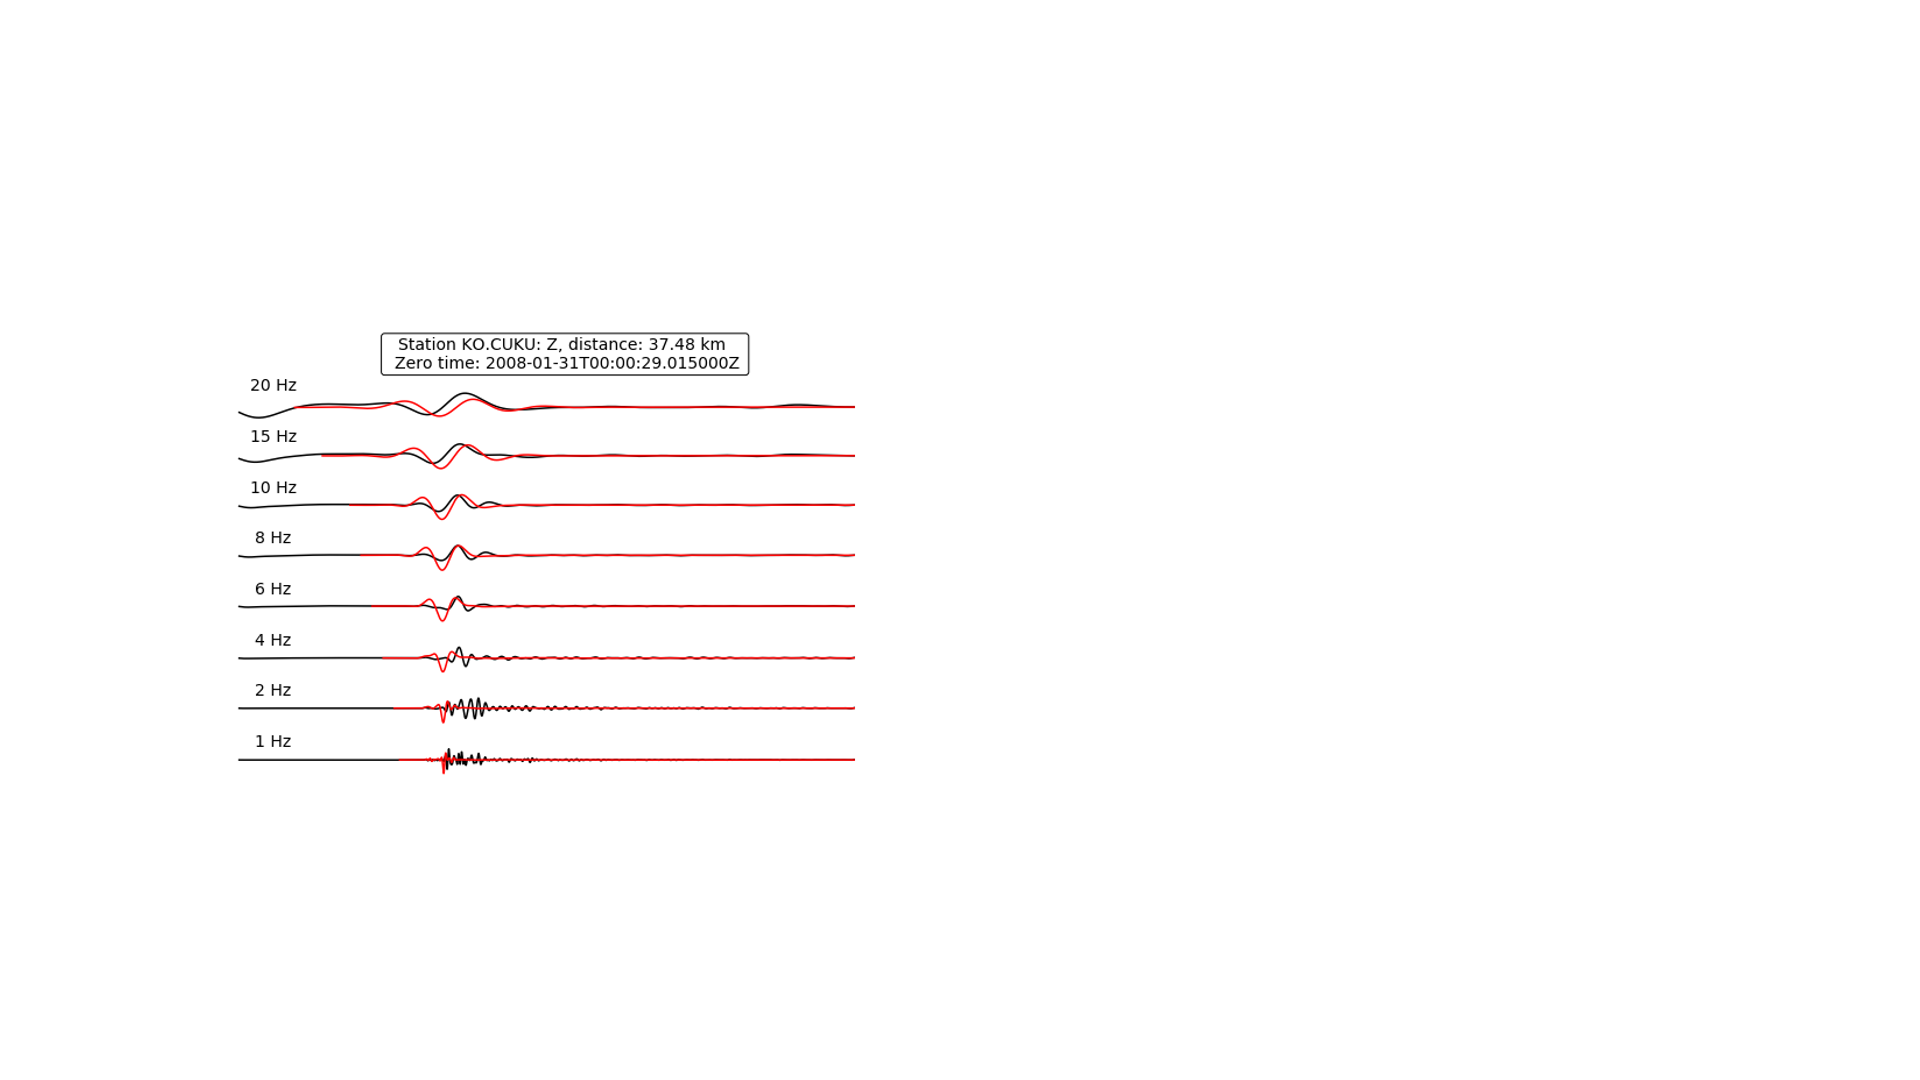
\includegraphics[width=0.5\linewith, trim = 5 cm 8 cm 20 cm 5 cm, clip]{images_results/manyfreqs.png}
    \caption{Caption}
    \label{fig:my_label}
\end{figure}


\begin{figure}
    \centering
    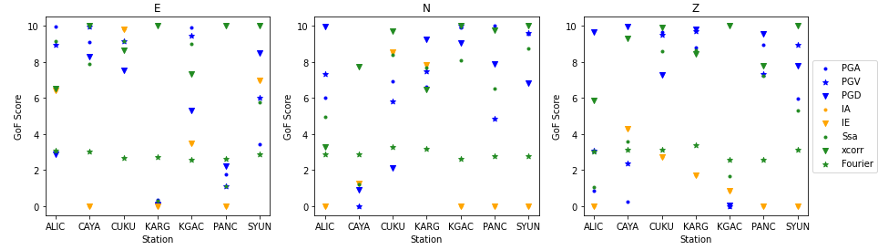
\includegraphics[width=\linewidth]{images_results/Gofsevenstations.png}
    \caption{Goodness of fit for the seven stations and all tested GoF parameters. \hl{Intend to change this for a figure that shows the change of fit with increasing frequency}}
    \label{fig:GoFsevenstations}
\end{figure}



\begin{sidewaysfigure}[!htp]
    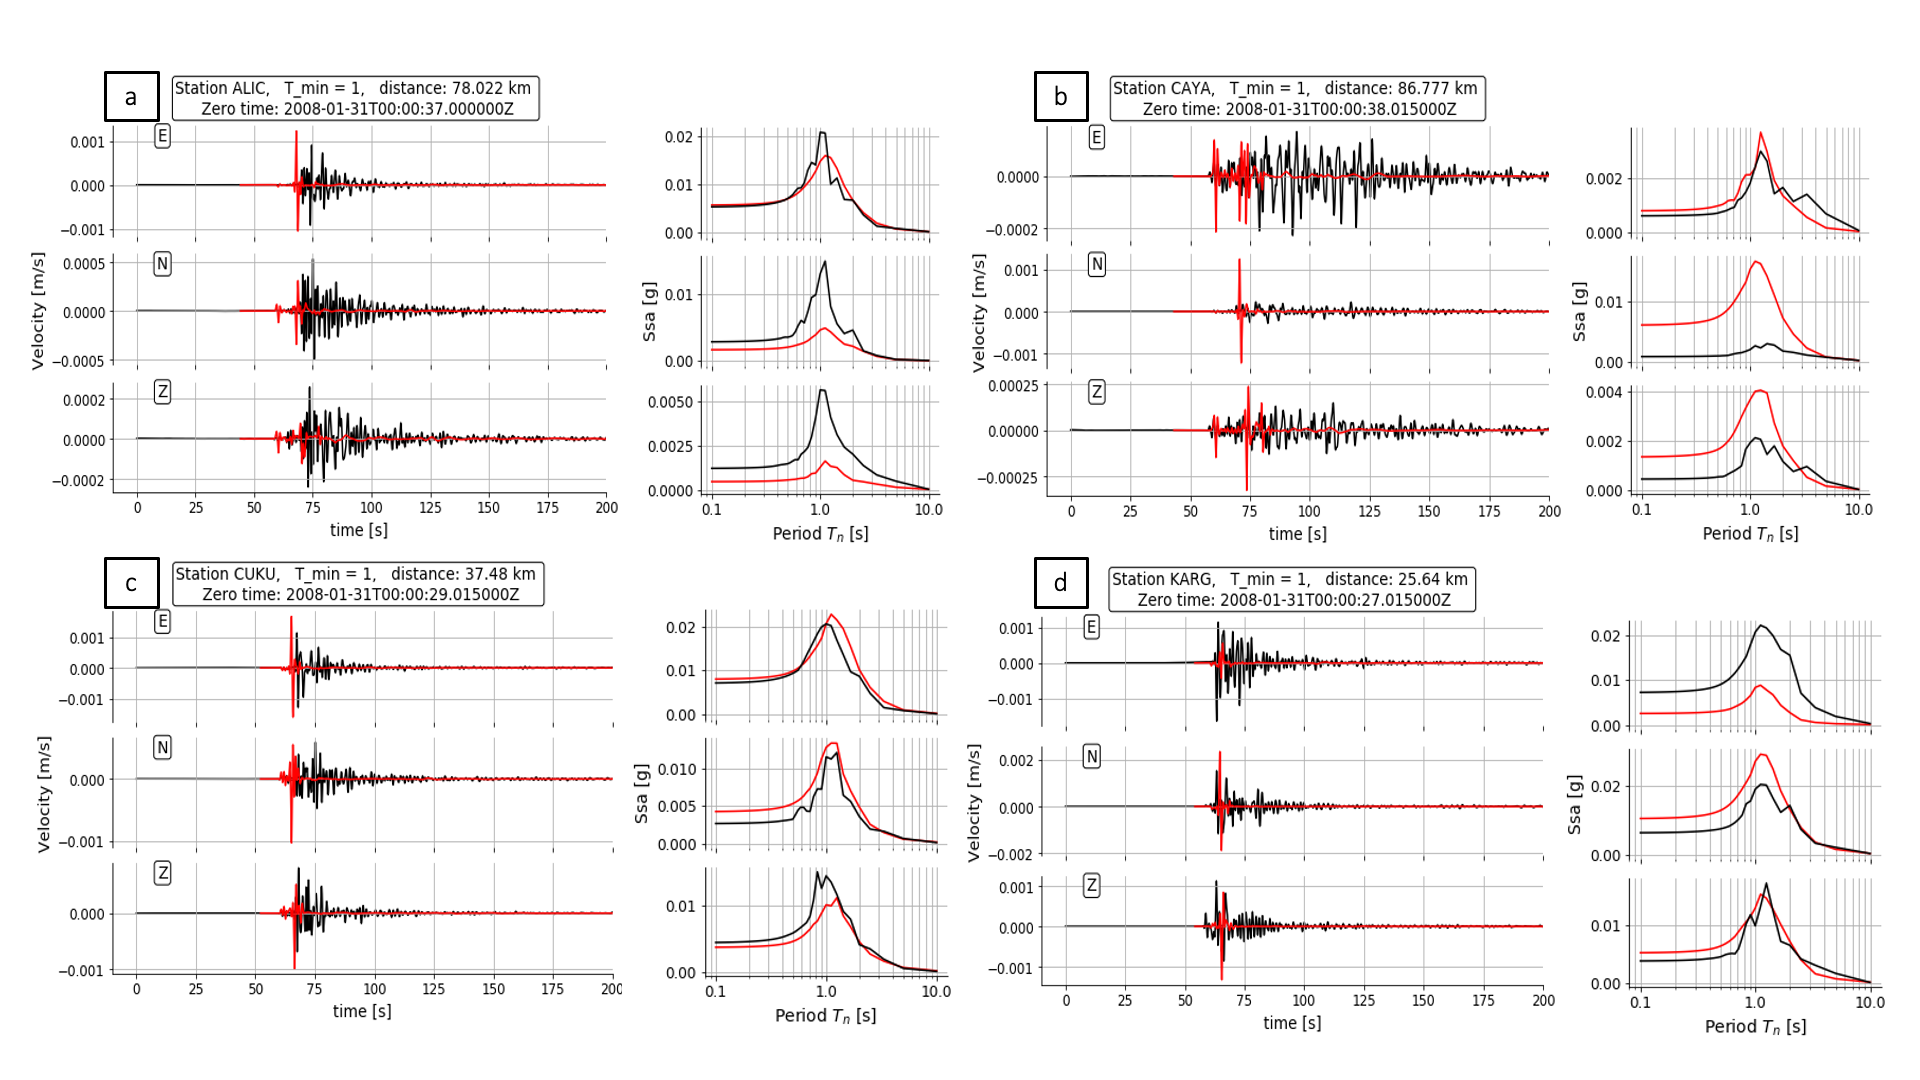
\includegraphics[width=\textwidth]{images_results/monsterfigure_part1.png}
  \caption{Velocity time series, Arias intensities and pseudo-spectral accelerations for all seven receivers, filtered at 1Hz. }
  \label{fig:monsterfigurea}
\end{sidewaysfigure}


\begin{sidewaysfigure}[!htp]

    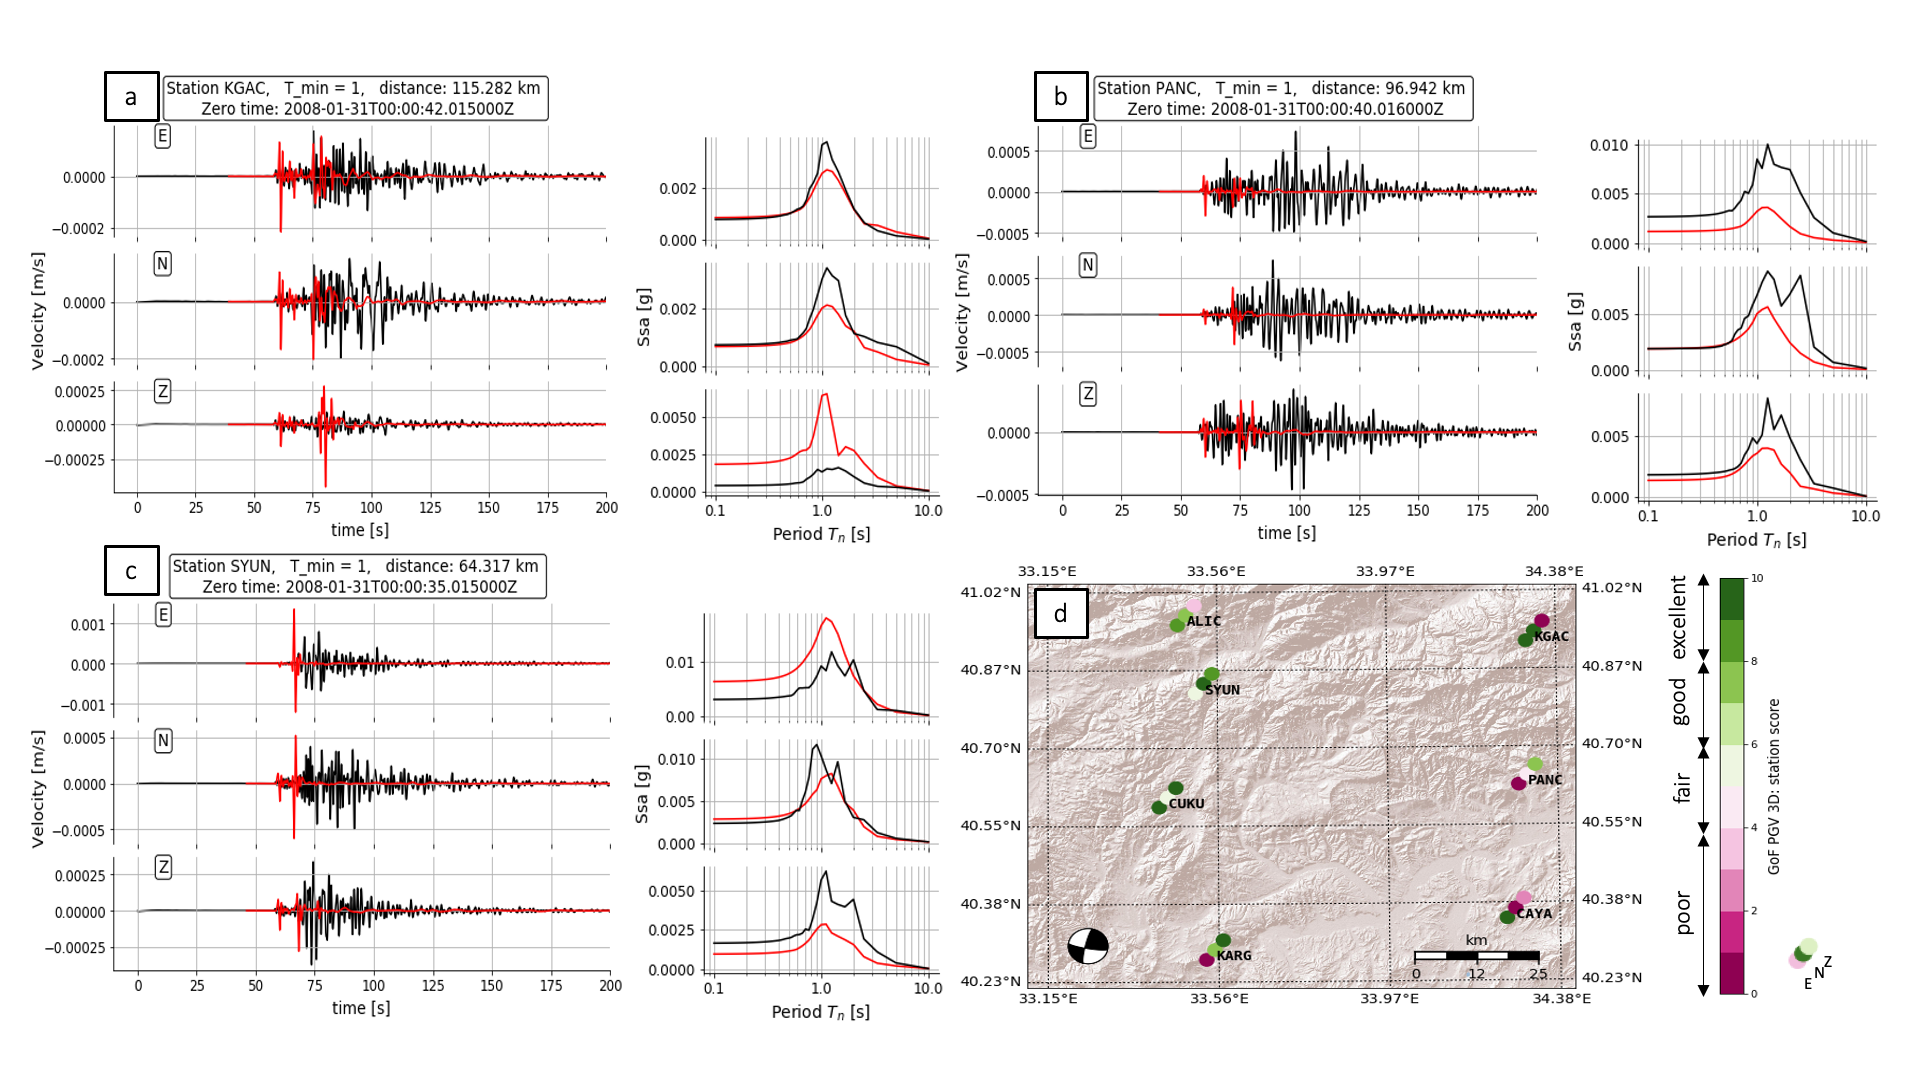
\includegraphics[width=\textwidth]{images_results/monsterfigure_part2.png}
  \caption{Velocity time series, Arias intensities and pseudo-spectral accelerations for all seven receivers, filtered at 1Hz.}
  \label{fig:monsterfigureb}
\end{sidewaysfigure}

\FloatBarrier

%%%%%%%%%%%%%%%%%%%%%%%%%%%%%%%%%%%%%%%%%%%%%%%%%%%%%%%%%%%%%%%%%%%%%%%%%%%%%%%%%%%%%%%%%%%%%%%%
%%%%%%%%%%%%%%%%%%%%%%%%%%%%%%%%%%%%%%.     .REF.     %%%%%%%%%%%%%%%%%%%%%%%%%%%%%%%%%%%%%%%%%%
%%%%%%%%%%%%%%%%%%%%%%%%%%%%%%%%%%%%%%%%%%%%%%%%%%%%%%%%%%%%%%%%%%%%%%%%%%%%%%%%%%%%%%%%%%%%%%%%

\section{Reference scenario and domain complexity}

In this section the results of the forward modelling in different domains are presented. In all cases, the 3D set-up is seen as the reference to which the other (1D, 3D + topo, 3D + topo + ocean) results are compared. The source is held at a constant location and depth of 10 km. From here on, only the PGV patterns will be shown. Appendix \ref{app:PGAsame} shows that the pattern for PGA is very similar to the PGV pattern for the more complex 3D + topo + ocean setting. 

\subsection{CMT1, perfect strike-slip}

Here we present the results for an event with an artificial magnitude of $M_0 = 1.0$. The reference event CMT1 consists of a perfect strike-slip source with strike, dip and rake as 90, 90, 180 (see Table \ref{tab:CMTstarts}). In this section, the differences between the reference event for the four proposed scenarios (1D, 3D, 3D + topo, 3D + topo + ocean) are evaluated and compared to the results of the 3D domain. 

Figure \ref{fig:ref_CMT1} shows the PGV distribution of the event for the E, N and Z orientations in the four domain types. Results are normalised over the 3D scenario in each direction. 

\begin{figure}[htp!]
    \centering
    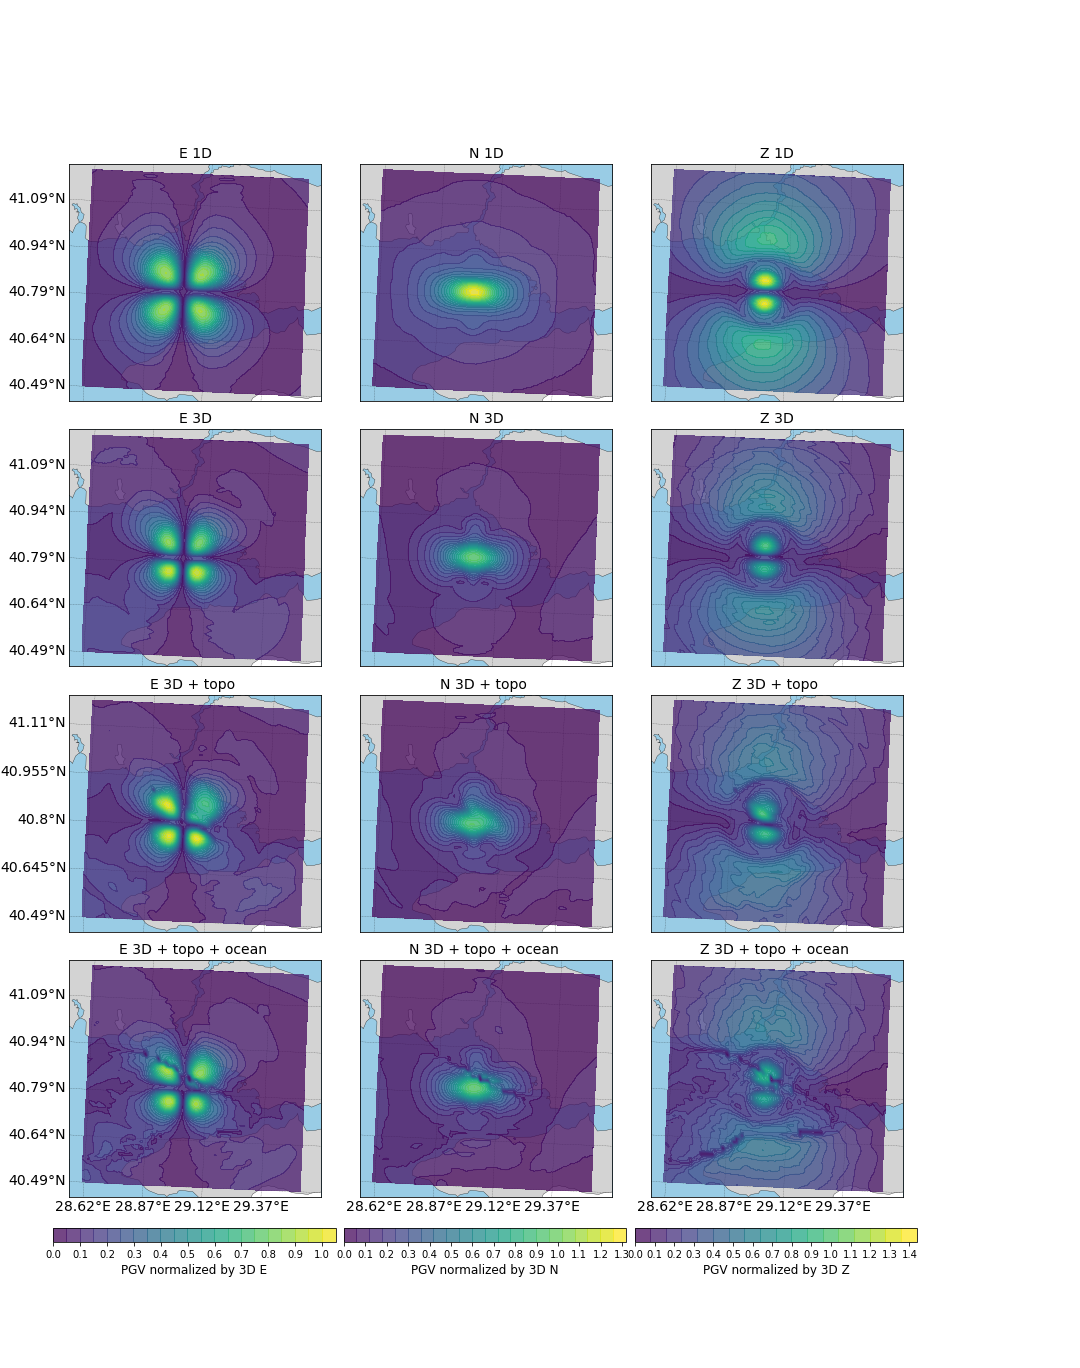
\includegraphics[width=1\linewidth, trim = 0cm 3cm 5.5cm 4cm, clip]{images_results/Ref_scenarios_normalized_sc1.png}
    \caption{PGV reference scenario CMT1, strike 90, dip 90, rake 180, normalised with respect to ref\_3D, meaning that it is normalised in E, N and Z directions separately with respect to the 3D flat model (second row).}
    \label{fig:ref_CMT1}
\end{figure}

\subsubsection{PGV pattern}

We first describe the 3D (second row) reference scenario. The reference shows a very clear pattern of the peak ground velocity that the perfect strike-slip mechanism has produced. Where the source imprint on the pattern is strong close to the source, it is more perturbed in the far field. The result of the spatial distribution of the PGV in the 1D domain (top row) is similar to the 3D result, and could be seen as a smoothed version of the 3D pattern. We see that the differences between the 3D and 1D model are in terms of maximum intensity close to the source (< 30 km), and beyond this point, the main differences are in the pattern. The peak PGV is intensified especially in the North and Z direction for the 1D model. This is in line with the results in the validation of Section \ref{sec:validation}, where the 1D model consistently over-estimates the 3D model. Topography, in the third row, has distorted the clear symmetry in the pattern as seen in the flat domains, especially along the steep ridge to the North-East of the source location. The effect is stronger in the horizontal directions than in the Z-direction. The PGV is amplified in the E and Z direction, and slightly de-amplified in the N direction. The influence on the far field remains similar to the patterns seen in the example without topography, however there is some intensification south and south-east of the source location on the mainland. The immediate observation in the ocean domain (bottom row) pattern is the influence of the mesh deformation where the simulated water layer stops and the ocean loading starts. Especially to the North-East of the source location, this effect is strong. The steep topography causing effects in the 3D + topography set-up is coinciding here with the change of ocean solid-fluid coupling and ocean loading.


\begin{figure}[htb!]%
    \centering
    \subfloat[]{{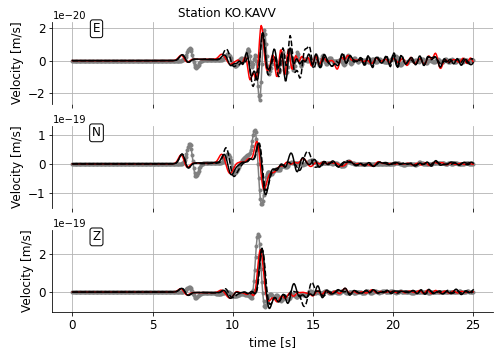
\includegraphics[width=7cm]{images_results/KAVV_scenario2.png} }}%
    %\qquad
    \subfloat[]{{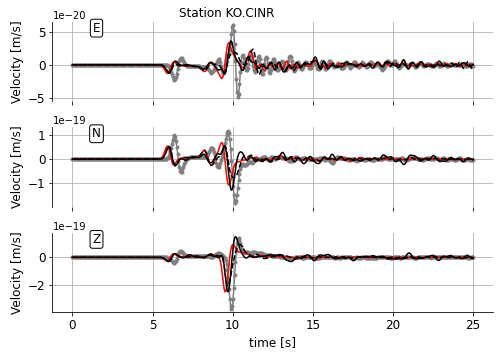
\includegraphics[width=7cm]{images_results/CINR_scenario2.png} }}%
    \qquad
    \subfloat[]{{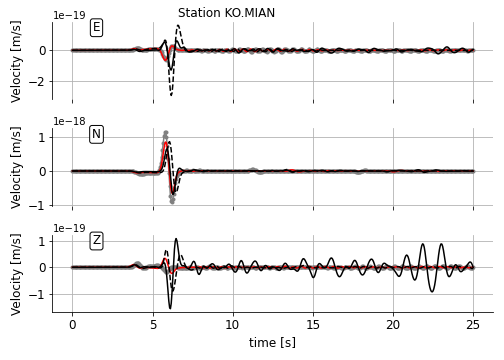
\includegraphics[width=7cm]{images_results/MIAN_scenario2.png} }}%
    %\qquad
    \subfloat[]{{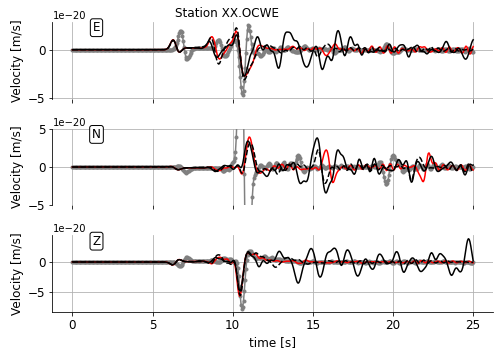
\includegraphics[width=7cm]{images_results/OCWE_scenario2.png} }}%
    %\qquad
    \caption{Records of the CMT1 event at four station locations, with dominant frequency 1 Hz. Stations KAVV(a), CINR(b), MIAN(c) are based on real station locations of the KOERI array and were selected from the closest location in the grid, station OCWE is chosen from a gridpoint towards the east located in the deeper Marmara sea, and is not based on a real station. Mind that the N component is clipped in y-direction to better display the effects of the ocean layer.}%
    \label{fig:CINRrecord_ref}%
\end{figure}

\subsubsection{Station records}

Records of this simulation at 1 Hz dominant frequency recorded by the KO stations KAVV (Istanbul), MIAN (near-fault island), and CINR (mainland south of Çinarcik) and are plotted in Figures \ref{fig:CINRrecord_ref} a-d. Station KAVV, located in Istanbul, shows a higher peak velocity for the 1D model with respect to the other models and is delayed for the first motions by 1 s. Likewise, the surface wave amplitude is higher for the 1D model result. The topography has additional velocity peaks at 15 s and after 25 s, and generally cause longer coda wave durations. These are de-amplified in the 3D+topo+ocean domain in the eastern direction. Station CINR, on the mainland south of the earthquake source, shows similar effects. The topography and ocean layer can be seen to cause a slight time lag here, especially in the north and vertical direction. Station MIAN sits at an interesting location, just above the steep rise in topography north-west of the source location. This is where the ocean-loading formulation is employed. Here, a very distinct signature of topography is visible in the east and vertical direction. The east signal is de-amplified in the ocean scenario, whereas the vertical signal is amplified. Significant reverberations in the coda wave are introduced by the ocean scenario.  The amplitudes in northern direction concur, with a slight delay caused by the topography. A non-existent receiver, here named XX.OCWE, is placed on the ocean to the east of the domain, to see further into the ocean effects. Here it becomes clear that the ocean affects primarily the coda of the wave, with large oscillations far beyond the main waveforms in E and Z direction. The coda revertebrations are the strongest in the north component, which is clipped for better displaying the ocean effect. Another feature that comes forward here is some type of multiple reflection at 16 and 22 seconds. Inclusion of topography shifts these signals to earlier times, and the ocean domain amplifies it to a larger amplitude than the main surface wave.

%%%%%%%% ----------------------- CMT2 ------------------------ %%%%%%%%%%

\subsection{CMT2 strike-slip}

\begin{figure}[htp!]
    \centering
    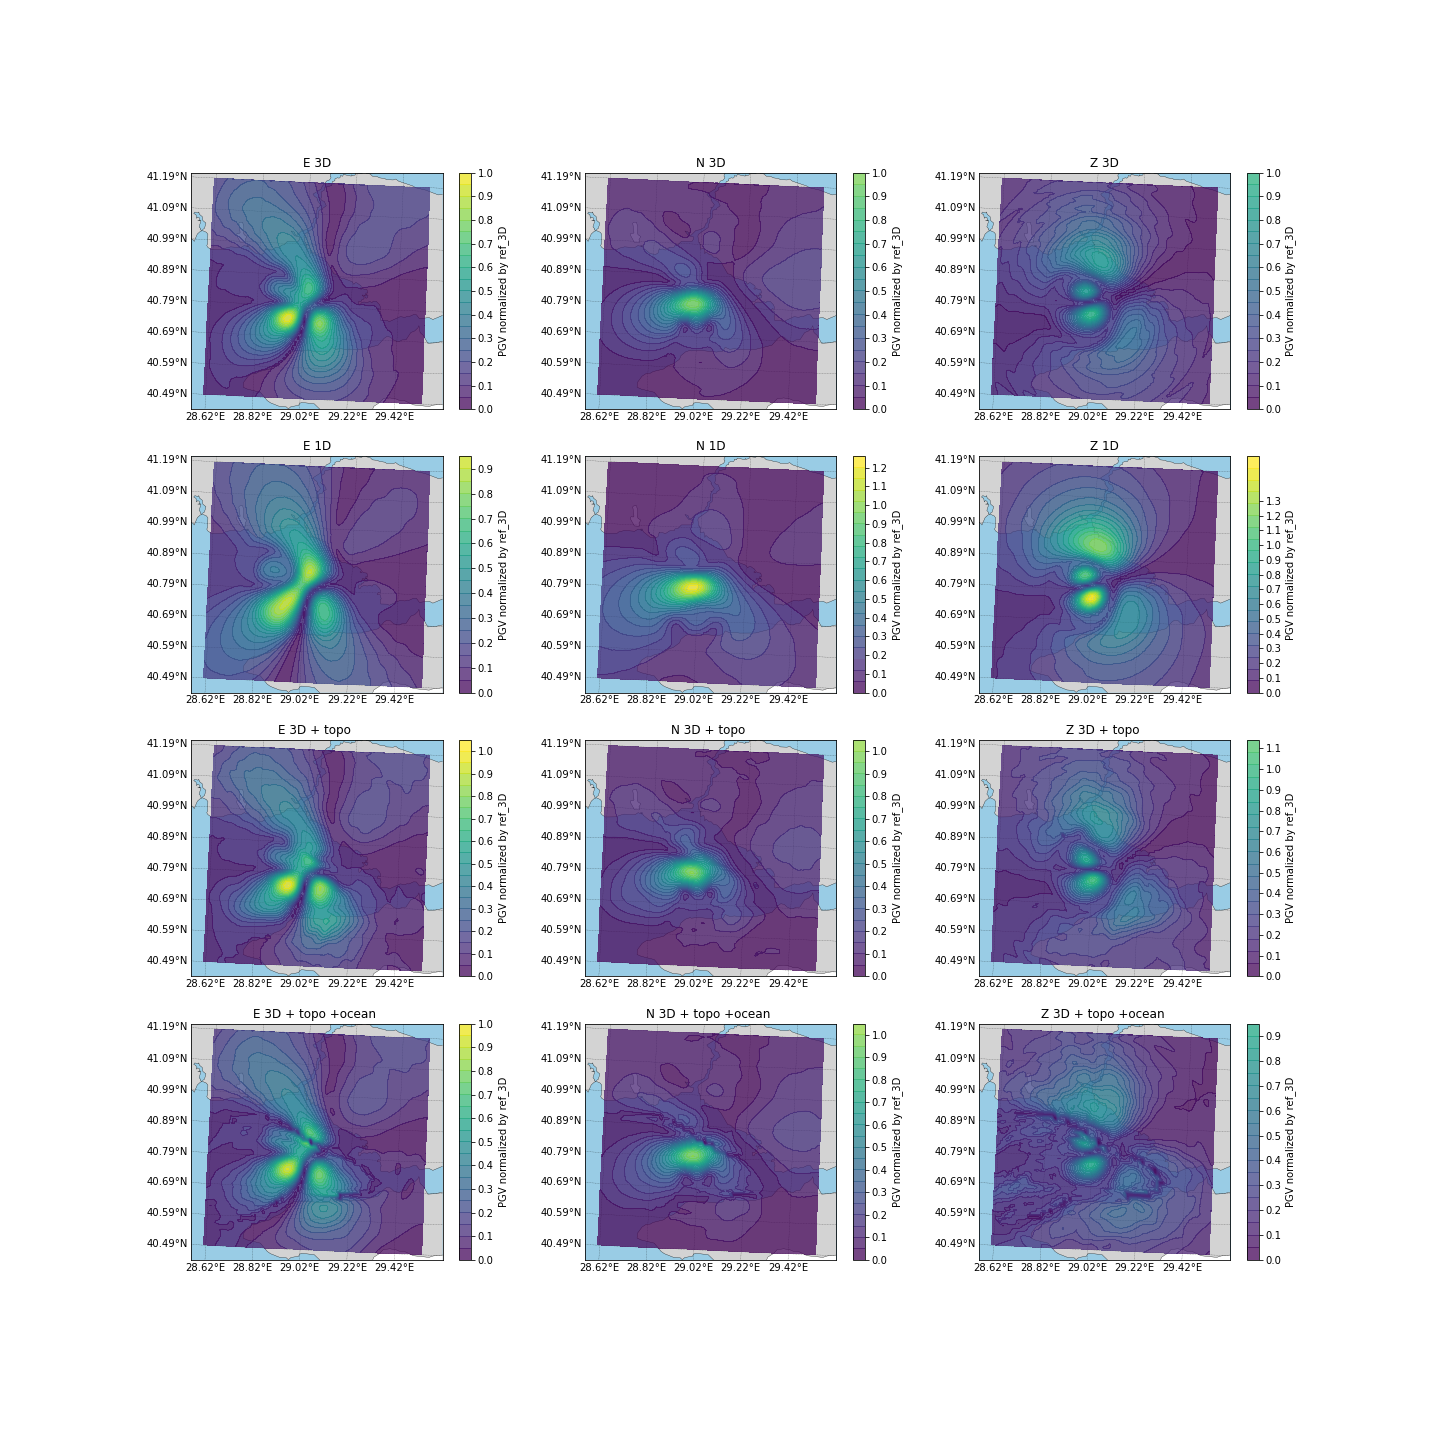
\includegraphics[width=1\linewidth, trim = 0cm 3.5cm 5.5cm 4cm, clip]{images_results/Ref_scenarios_normalized_sc2.png}
    \caption{PGV reference scenario CMT2, strike 100, dip 75, rake 160, normalized with respect to the 3D configuration (top row).}
    \label{fig:ref_CMT2}
\end{figure}

Another strike-slip scenario (CMT2) is tested: now with a slightly tilted strike (100 $\degree$), a less steep dip (75 $\degree$) and a rake that indicates a slightly more oblique faulting mechanism (160 $\degree$), see Table \ref{tab:CMTstarts}. The main motivation for this is to remain in a dextra strike-slip regime that is realistic for the NAFZ, but starts from a starting point that does not involve fractions of $\frac{\pi}{2}$, to avoid zeros in the moment tensor components (see Appendix \ref{app:sdrvar_methods}).

We start with the 1D domain, which is now less symmetric then the perfect strike-slip case considered above, although the patterns are still recognisable. With the rake pointing more to the south-west, the peak velocities are directed towards the south now. Similar observations can be made for the 3D model, which shows a perturbed version of the 1D result, and de-amplifies the north and vertical component as well as amplifying the east component. Inclusion of topography has less influence on the northern part of the domain now, because most of the energy is sent southward, away from the steep ridge. Some amplification takes in the south near Çinarcik, where the waveforms come onto land. The ocean has an effect especially more towards the deep part of the Marmara sea in the east. 


\subsection{More CMT starting configurations}

Even though the fault at question is characterised as a strike-slip fault, we have tested two other configurations: CMT3 and CMT4 (see Table \ref{tab:CMTstarts}). These other two starting configurations comprise a normal (CMT3) and thrust (CMT4) regime. The motivation behind this was to test whether the effects observed were unique to a strike-slip configuration, or if these observations could be consistent for other types of faulting. The resulting images of these two configurations are displayed in Appendix \ref{app:morereffigs}. Here the same holds true: the 1D model is a smoothed version of the 3D model result, and amplifies the PGV. The steep topography distorts the PGV pattern close to the source and the imprint of the ocean simulation edge can be seen in the 3D + topo + ocean figures. 

\hl{To do: include traces and perhaps a spectrum showing the differences between the 4 model types}


%An overview of the four domain types for the reference scenario is given in Figure (\hl{paraview image of four domain types?}). 

\FloatBarrier

%%%%%%%%%%%%%%%%%%%%%%%%%%%%%%%%%%%%%%%%%%%%%%%%%%%%%%%%%%%%%%%%%%%%%%%%%%%%%%%%%%%%%%%%%%%%%%%%
%%%%%%%%%%%%%%%%%%%%%%%%%%%%%%%%%%%%%  .VARIATION.   %%%%%%%%%%%%%%%%%%%%%%%%%%%%%%%%%%%%%%%%%%%
%%%%%%%%%%%%%%%%%%%%%%%%%%%%%%%%%%%%%%%%%%%%%%%%%%%%%%%%%%%%%%%%%%%%%%%%%%%%%%%%%%%%%%%%%%%%%%%%

\section{Moment tensor component variation}

In this section we deviate from the CMT starting configurations as stated in Table \ref{tab:CMTstarts}. The coefficient of variation $\text{Cv}$ is calculated for variation of strike, dip and rake in the four different domain types. 

\subsection{strike}

\subsubsection{CMT1}

\begin{figure}[!htb]
    \centering
    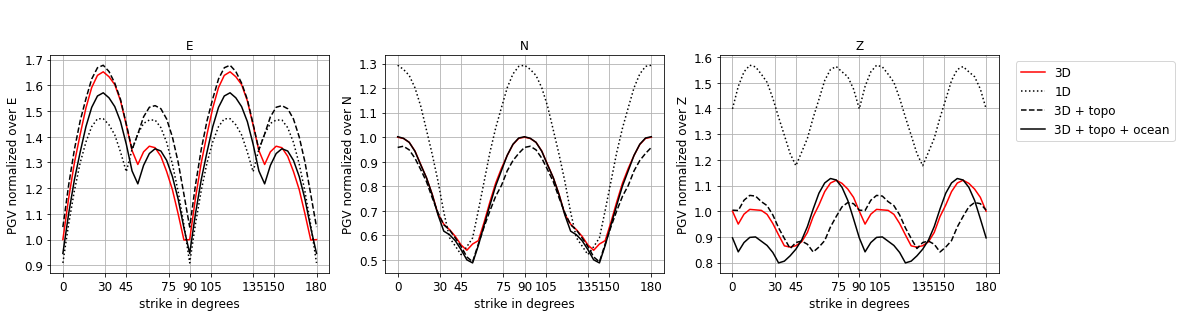
\includegraphics[width=\textwidth]{images_results/fullrange_strikevar_maxvals_sc1.png}
    \caption{Full 180$\degree$ range strike variation of the maximum measured PGV. Starting configuration CMT1: dip 90$\degree$, rake 180$\degree$}
    \label{fig:KAVV_fullrange_1}
\end{figure}

The strike has a range of 0 to 180$\degree$ total. It is varied here for 45$\degree$ in each direction. Figure \ref{fig:ref_sigma1_strike} shows the coefficient of variation $\text{Cv}$ with respect to each domain and starting scenario. E.g. for PGV N 3D + topo, the coefficient of variation is calculated with respect to the values of the reference scenario of PGV N 3D + topo. For the E and Z directions, the main and largest peak velocity variations take place along the initial strike of the fault. The north component shows a stronger variation near the +/- 45$\degree$ strike end-members of the variation. The 1D model in this case tells a very different story than the 3D models. It shows very symmetrical patterns compared to the simulations that made use of the 3D model. The lateral variations in the velocity model seem to cause more variation in the North-West section of the grid. The topography in the 3D + topo and 3D + topo + ocean scenarios has a significant damping effect of close to an order of magnitude on the velocity variations in the N and Z directions especially. The E direction for these scenarios shows a slightly perturbed result of the 3D model. The direct imprint of the edge of ocean coupling is less visible in this case and seems to have little influence on the variations. 

\begin{figure}[htb]
    \centering
    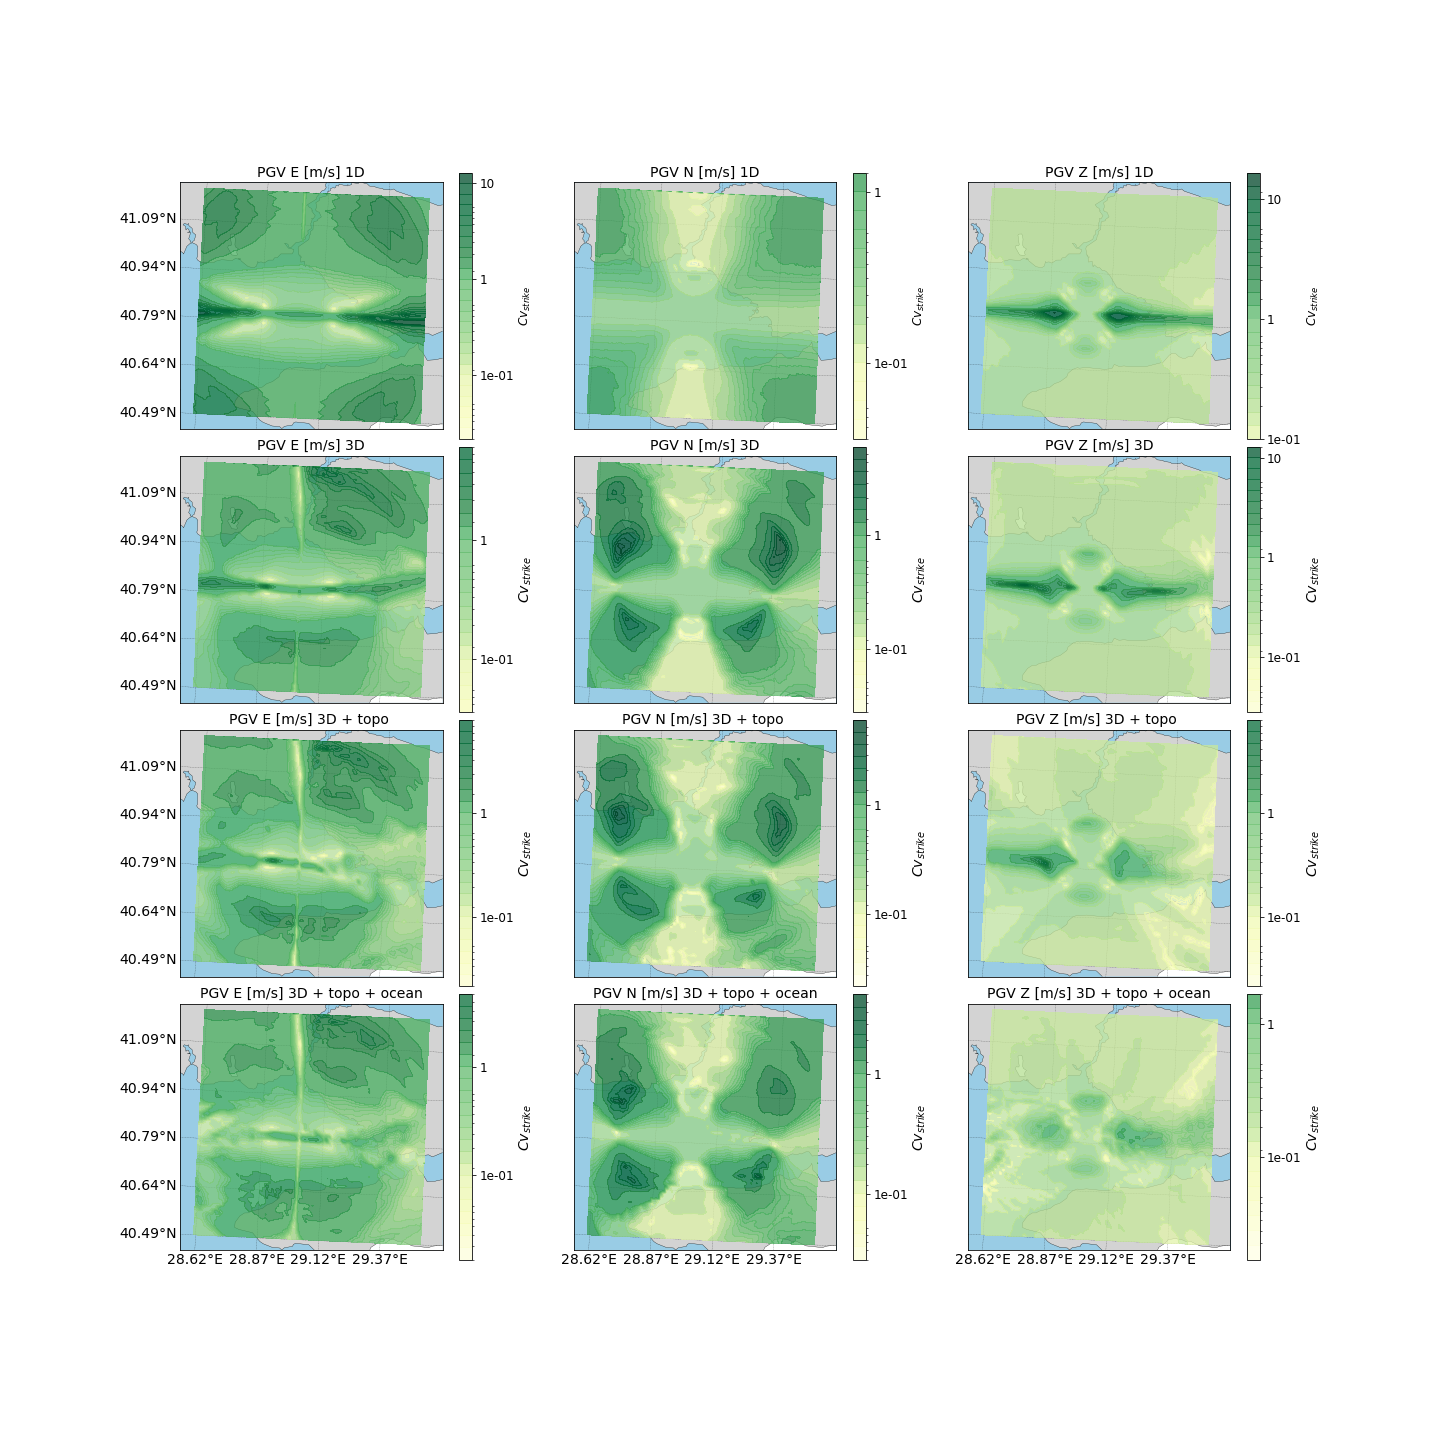
\includegraphics[width=1\linewidth, trim = 2cm 5cm 1cm 5cm, clip]{images_results/strike_variation_sigma_sc1.png}
    \caption{CMT1 coefficient of variation $Cv$ of strike variation, for each model domain in E, N and Z direction. Colourbar set to logarithmic to adequately show the large differences.}
    \label{fig:ref_sigma1_strike}
\end{figure}

\FloatBarrier
% check ff of dit klopt of het KAVV is

Figures \ref{fig:ref_eps12-1} and \ref{fig:ref_eps25-1} show the relative difference between the strike varied $- 11.25\degree$ and $- 22.5\degree$, respectively. What becomes clear here is that the 1D domain amplifies in the E and Z directions, but de-amplifies in the N direction perpendicular to the fault strike. For the doubling of the strike angle, the maximum relative difference also doubles. A striking feature is the consistency of the difference pattern. The largest differences seem to concentrate along the initial 100$\degree$ fault strike for the N and Z components, and at an angle of 45$\degree$ with the initial fault strike for the N component. As the angle of the fault progresses from 11.25$\degree$ to the double 22.5$\degree$, this pattern remains unchanged and intensifies in these locations. 

The normalised PGV for the full range of strike variation (0$\degree$-180$\degree$) is plotted in Figure \ref{fig:KAVV_fullrange_1}. This periodic pattern supports that mainly the 1D pattern is exhibiting much higher peak velocities in N and Z directions at this point. Where the maximum PGV is symmetric around 90 $\degree$ for the 1D model in E and Z, it is not for the 3D, 3D + topo and 3D + topo + ocean. The other scenarios are all in close range to each other. The 1D symmetry could be attributed to the lack of lateral variations in the velocity model. Topography and ocean seem to have an influence mainly on the E and Z directions. The periodic pattern in E, N and Z direction could be linked to the general pattern of the influence of strike dip and rake on the moment tensor pattern starting from the CMT1, as presented in Appendix \ref{app:sdrvar_methods}. As PGV is defined as the absolute maximum of the time series, the values are only positive in the full range figure here. 

\begin{figure}[!htb]
    \centering
    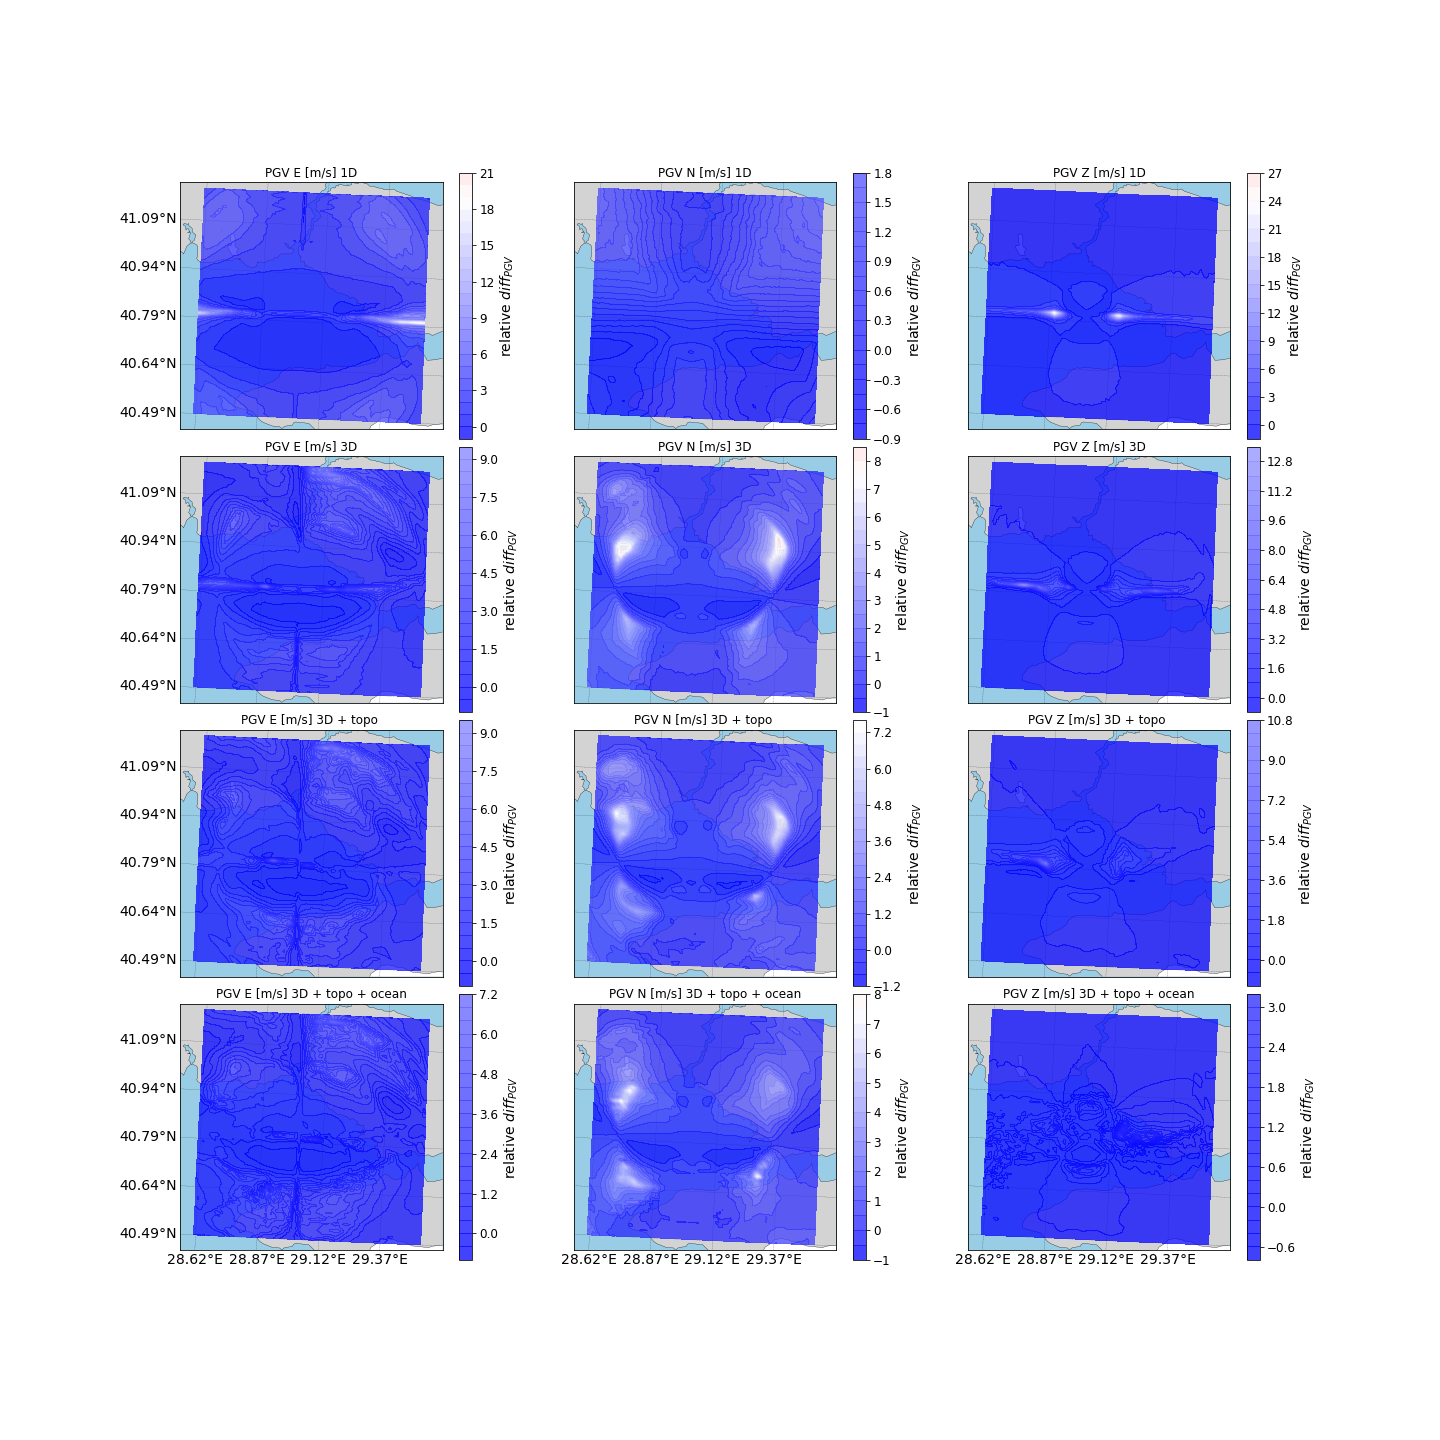
\includegraphics[width=1\linewidth, trim = 2cm 5cm 1cm 5cm, clip]{images_results/strike_variation_epsilon12_sc1.png}
    \caption{CMT1 relative difference between a scenario with a strike variation of 11.25$\degree$ with respect to the reference scenario. Colourbar set to the total minima and maxima of the 11.25$\degree$ and 22.5$\degree$ plots for comparison.}
    \label{fig:ref_eps12-1}
\end{figure}

\begin{figure}[h]
    \centering
    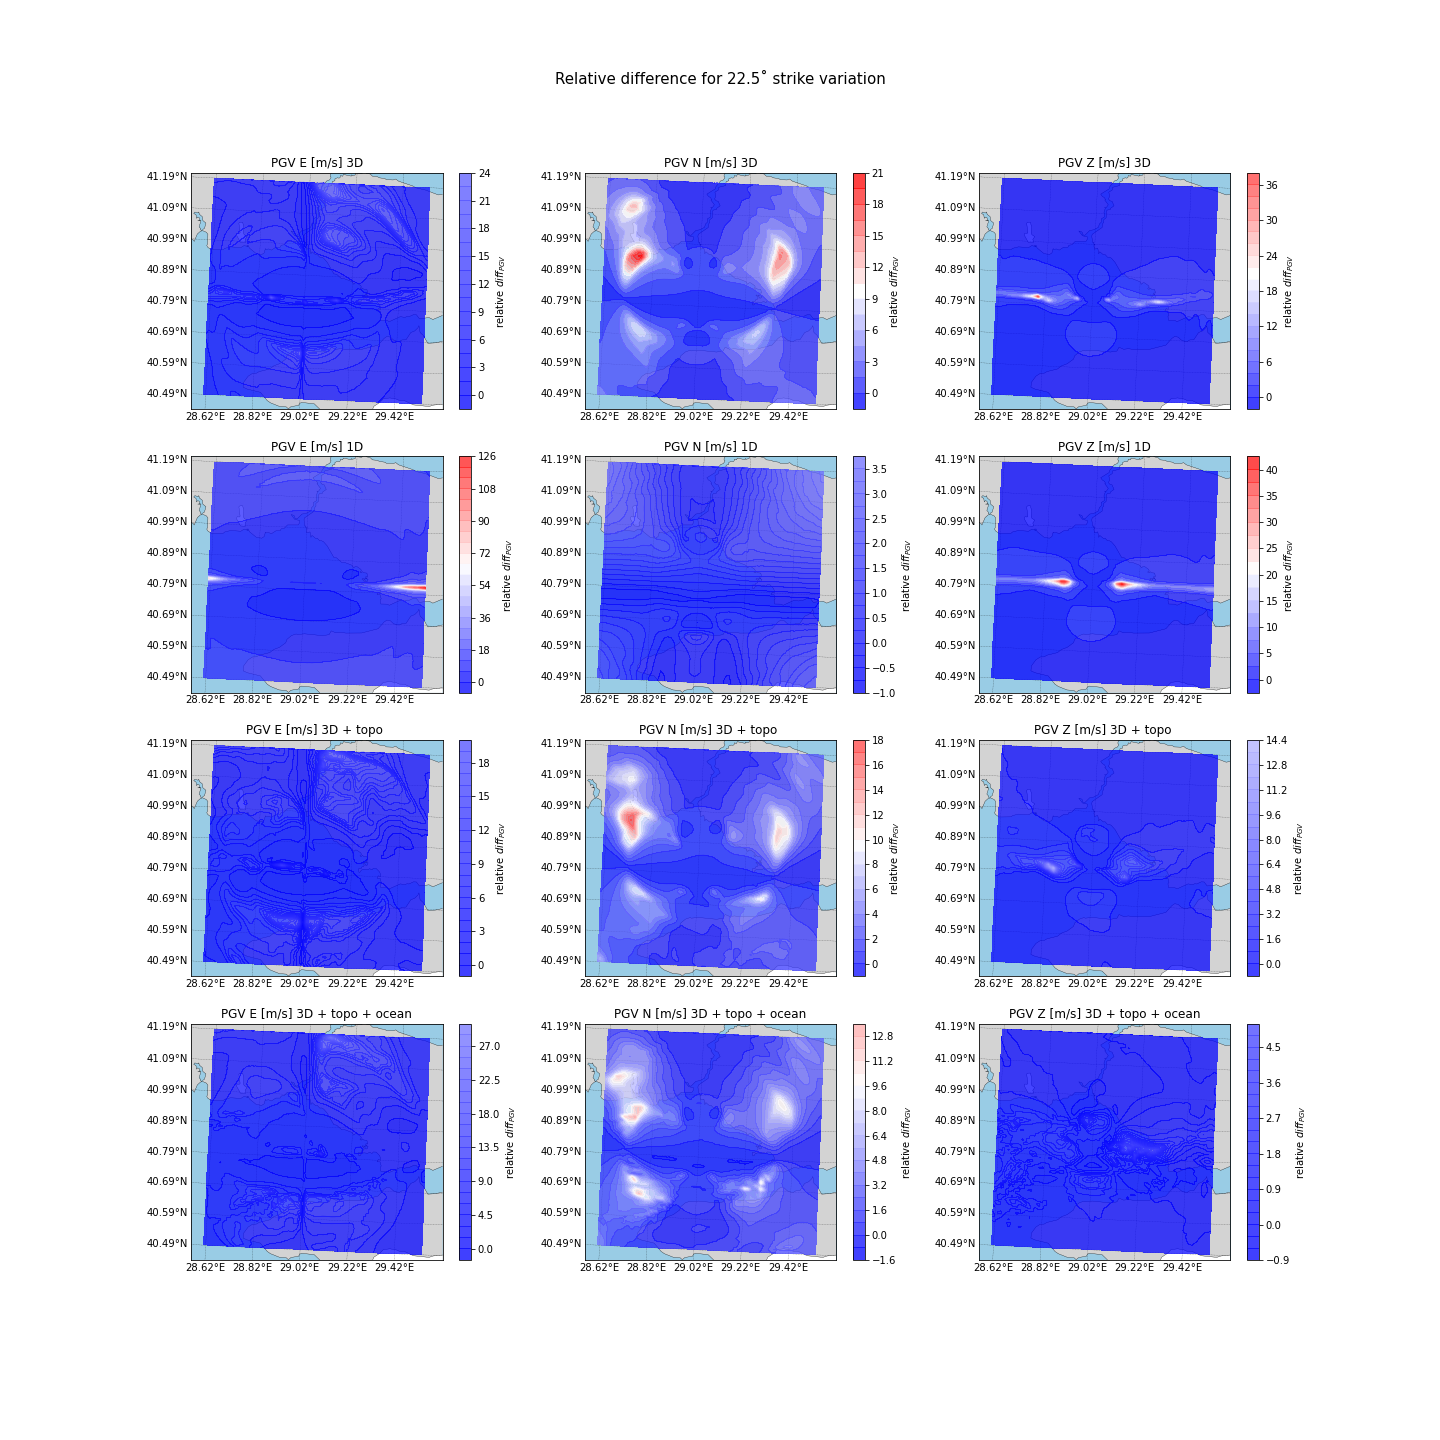
\includegraphics[width=1\linewidth, trim = 2cm 5cm 1cm 5cm, clip]{images_results/strike_variation_epsilon25_sc1.png}
    \caption{CMT1 relative difference between a scenario with a strike variation of 22.5$\degree$ with respect to the reference scenario. Colourbar set to the total minima and maxima of the 11.25$\degree$ and 22.5$\degree$ plots for comparison.}
    \label{fig:ref_eps25-1}
\end{figure}

\FloatBarrier

\subsubsection{CMT2}

\begin{figure}[!htp]
    \centering
    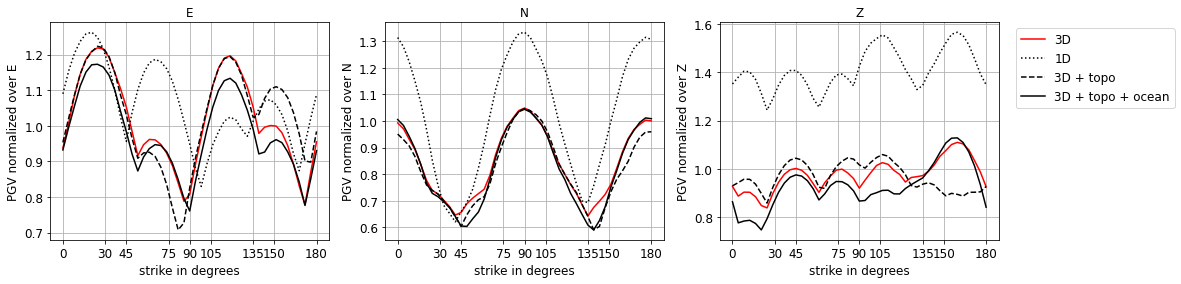
\includegraphics[width=0.8\textwidth]{images_results/fullrange_strikevar_maxvals_sc2.png}
    \caption{CMT2 Full 180$\degree$ range variation of the strike measured at station KAVV.}
    \label{fig:KAVV_fullrange_2}
\end{figure}

The same is evaluated for the CMT2 starting configuration. The $Cv$ in Figure \ref{fig:cmt2sigm} now shows less symmetrical patterns than the simple CMT1 starting case. This could be attributed to the different dip and rake starting point, which alter the variation of the total moment tensor (\hl{To do: supporting figure in methods for strike/dip/rake variations and influence on the total moment tensor}). The same trends as in CMT1 with respect to de-amplification of the variation influence in the 3D + topo and 3D + topo + ocean scenarios can be observed. The doubling of relative difference between the 11.25$\degree$ varied and 22.5$\degree$ varied strike still holds here. The full range in Figure \ref{fig:KAVV_fullrange_2} shows the same trend as CMT1: the 3D models are in similar ranges, the 1D shows higher peak velocity. Because the results are similar, the next sections will only contain images of the CMT2 3D configuration. The complete images can be found in Appendices \ref{figapp: strikevar}, \ref{figapp: dipvar} , \ref{figapp: rakevar}.


\begin{figure}[!htp]
    \centering
    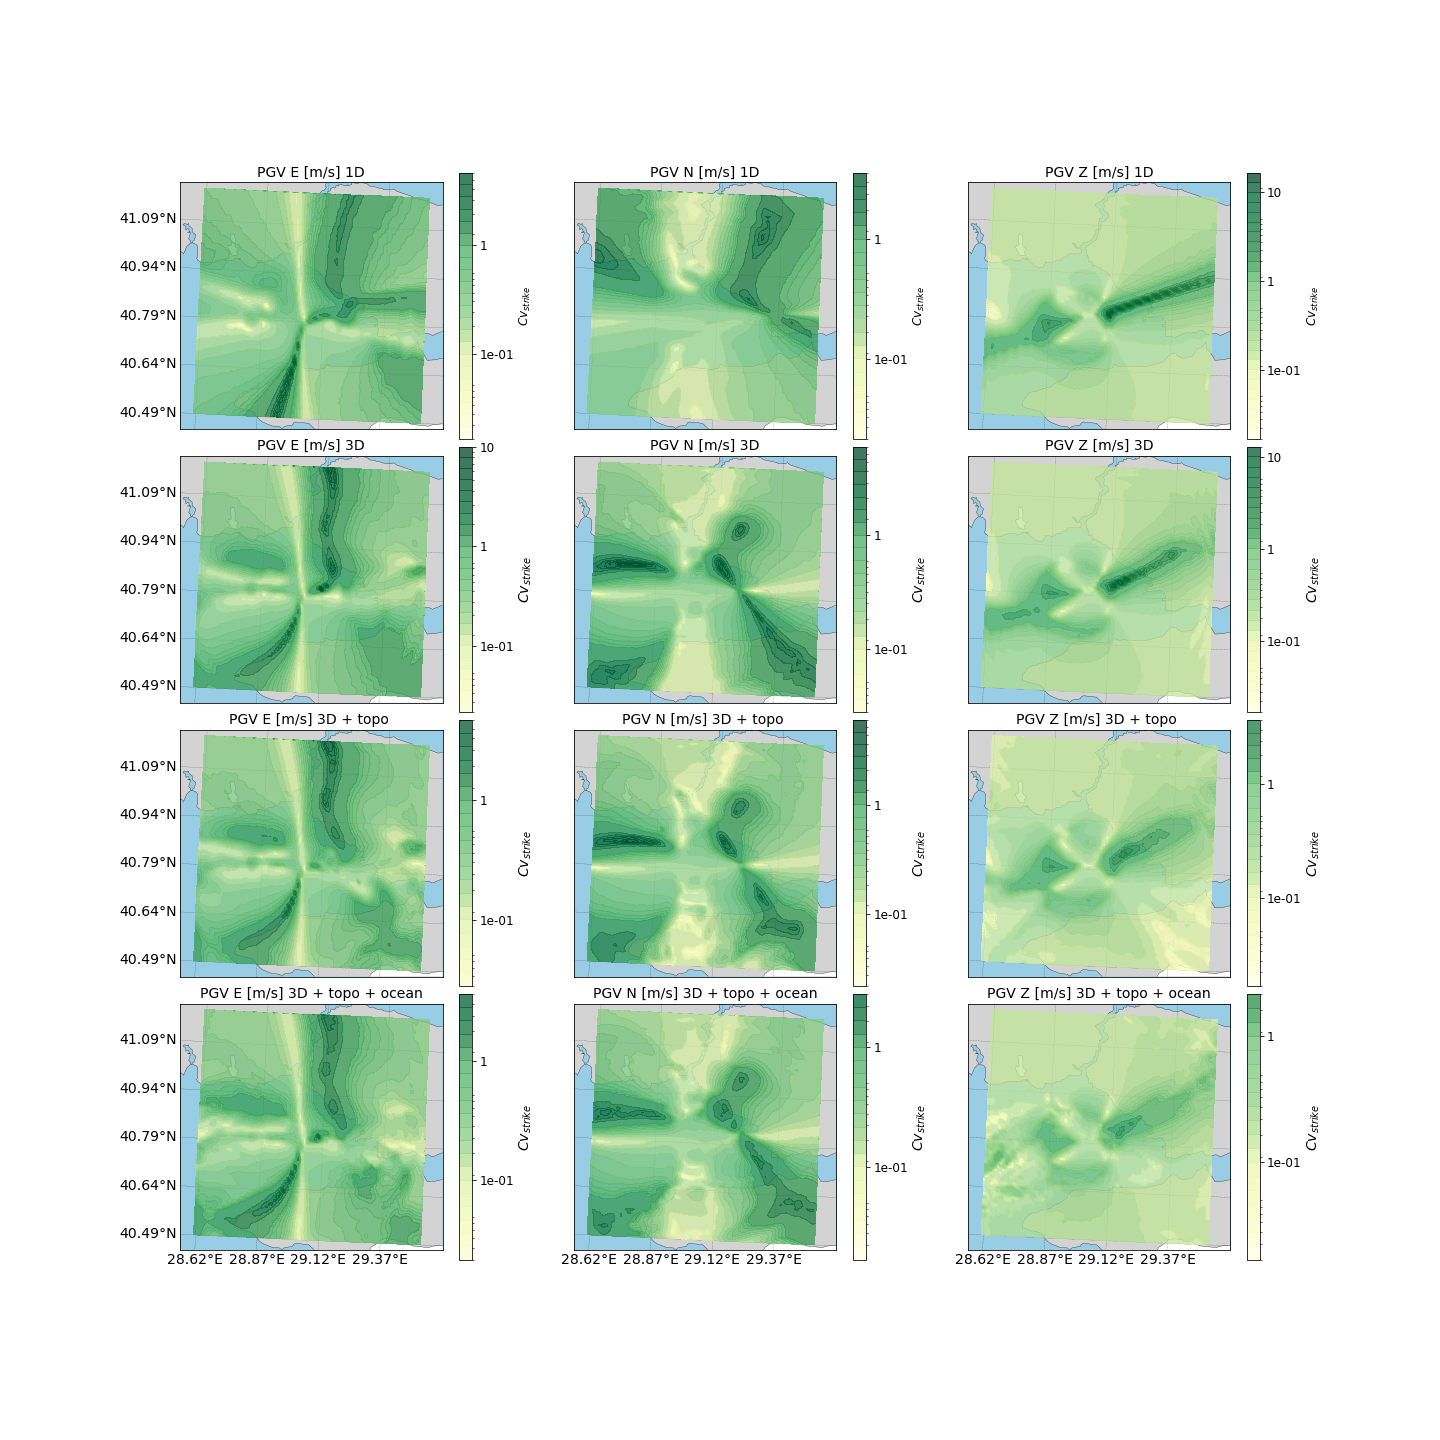
\includegraphics[width=1\linewidth,trim = 2cm 5cm 1cm 5cm, clip]{images_results/strike_variation_sigma_sc2.png}
    \caption{CMT2 coefficient of variation $\text{Cv}$ of strike variation, for each model domain in E, N and Z direction. Colourbar set to logarithmic to adequately show the large differences.}
    \label{fig:cmt2sigm}
\end{figure}



\begin{figure}[!htp]
    \centering
    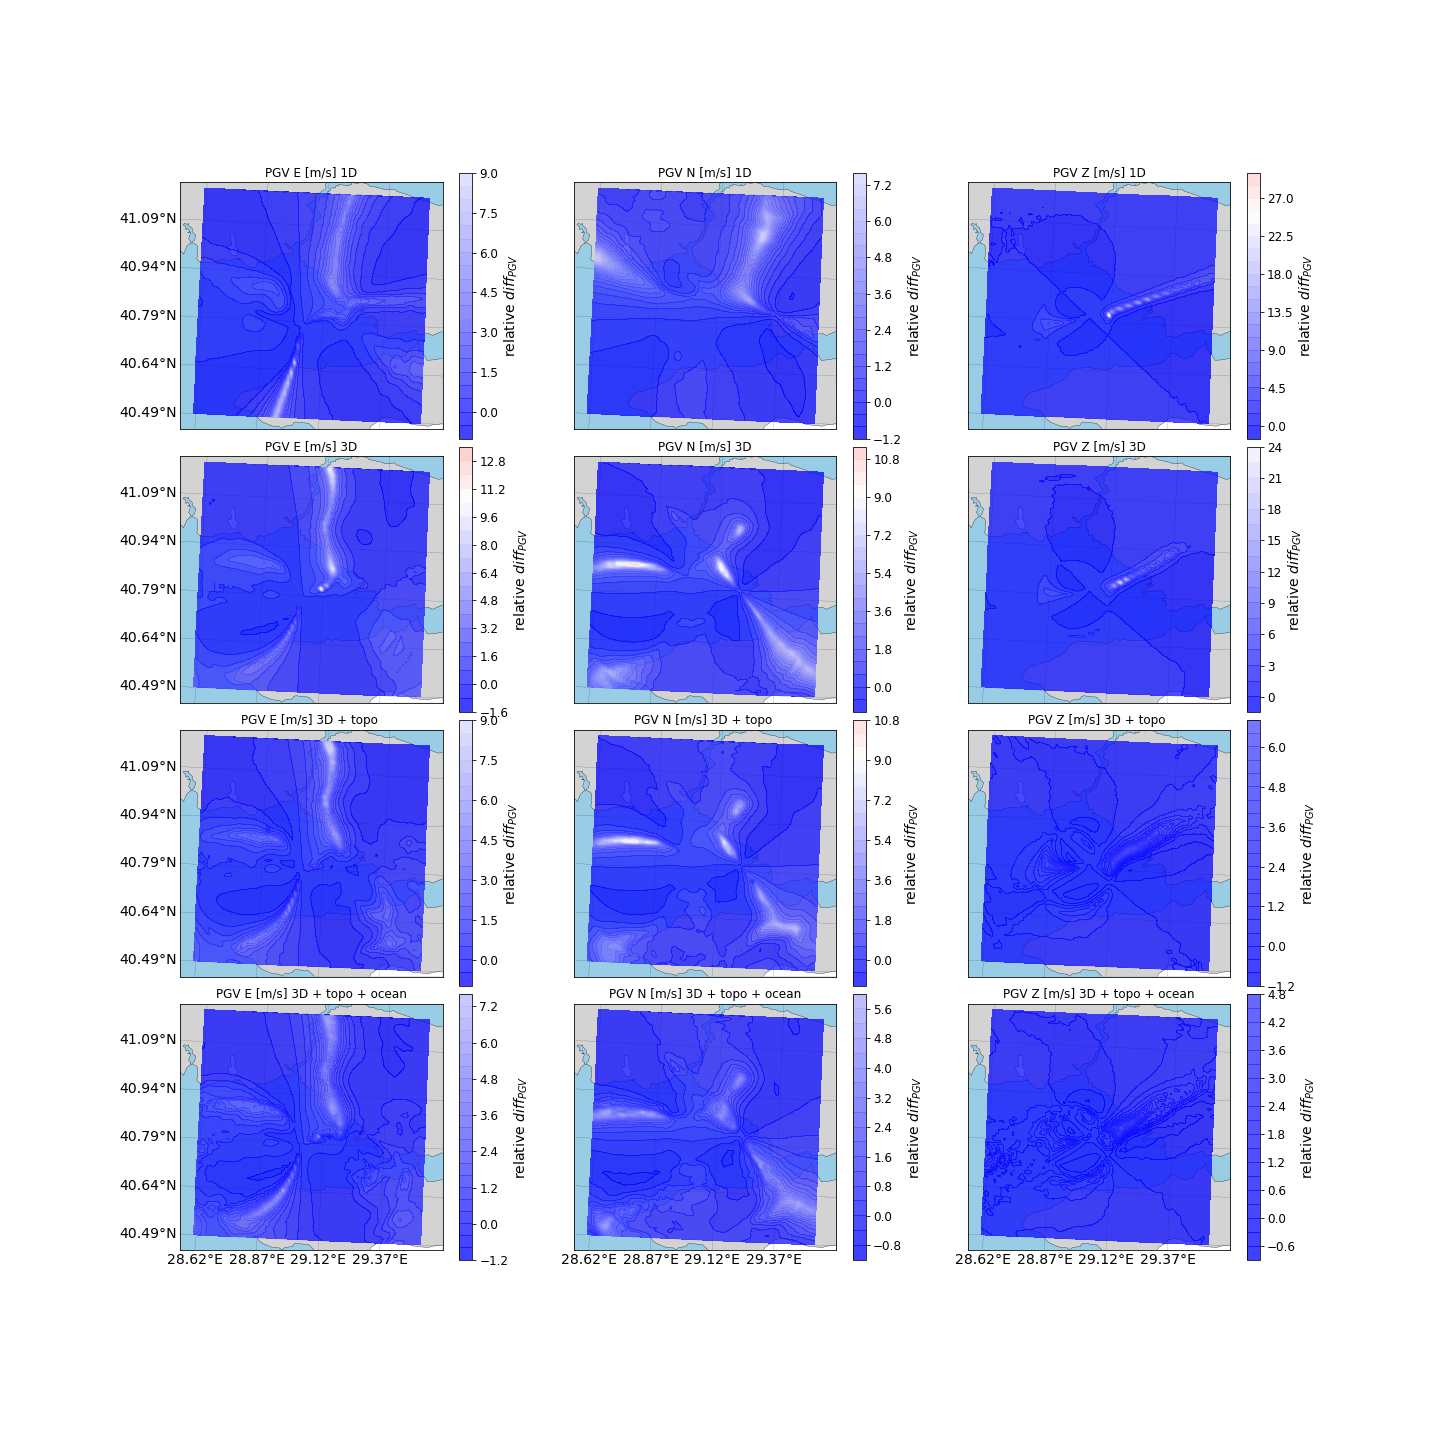
\includegraphics[width=1\linewidth ,trim = 2cm 5cm 1cm 5cm, clip]{images_results/strike_variation_epsilon12_sc2.png}
    \caption{CMT2 relative difference between a scenario with a strike variation of 11.25$\degree$ with respect to the reference scenario. Colourbar set to the total minima and maxima of the 11.25$\degree$ and 22.5$\degree$ plots for comparison.}
    \label{fig:ref_eps12-2}
\end{figure}

\begin{figure}[!htp]
    \centering
    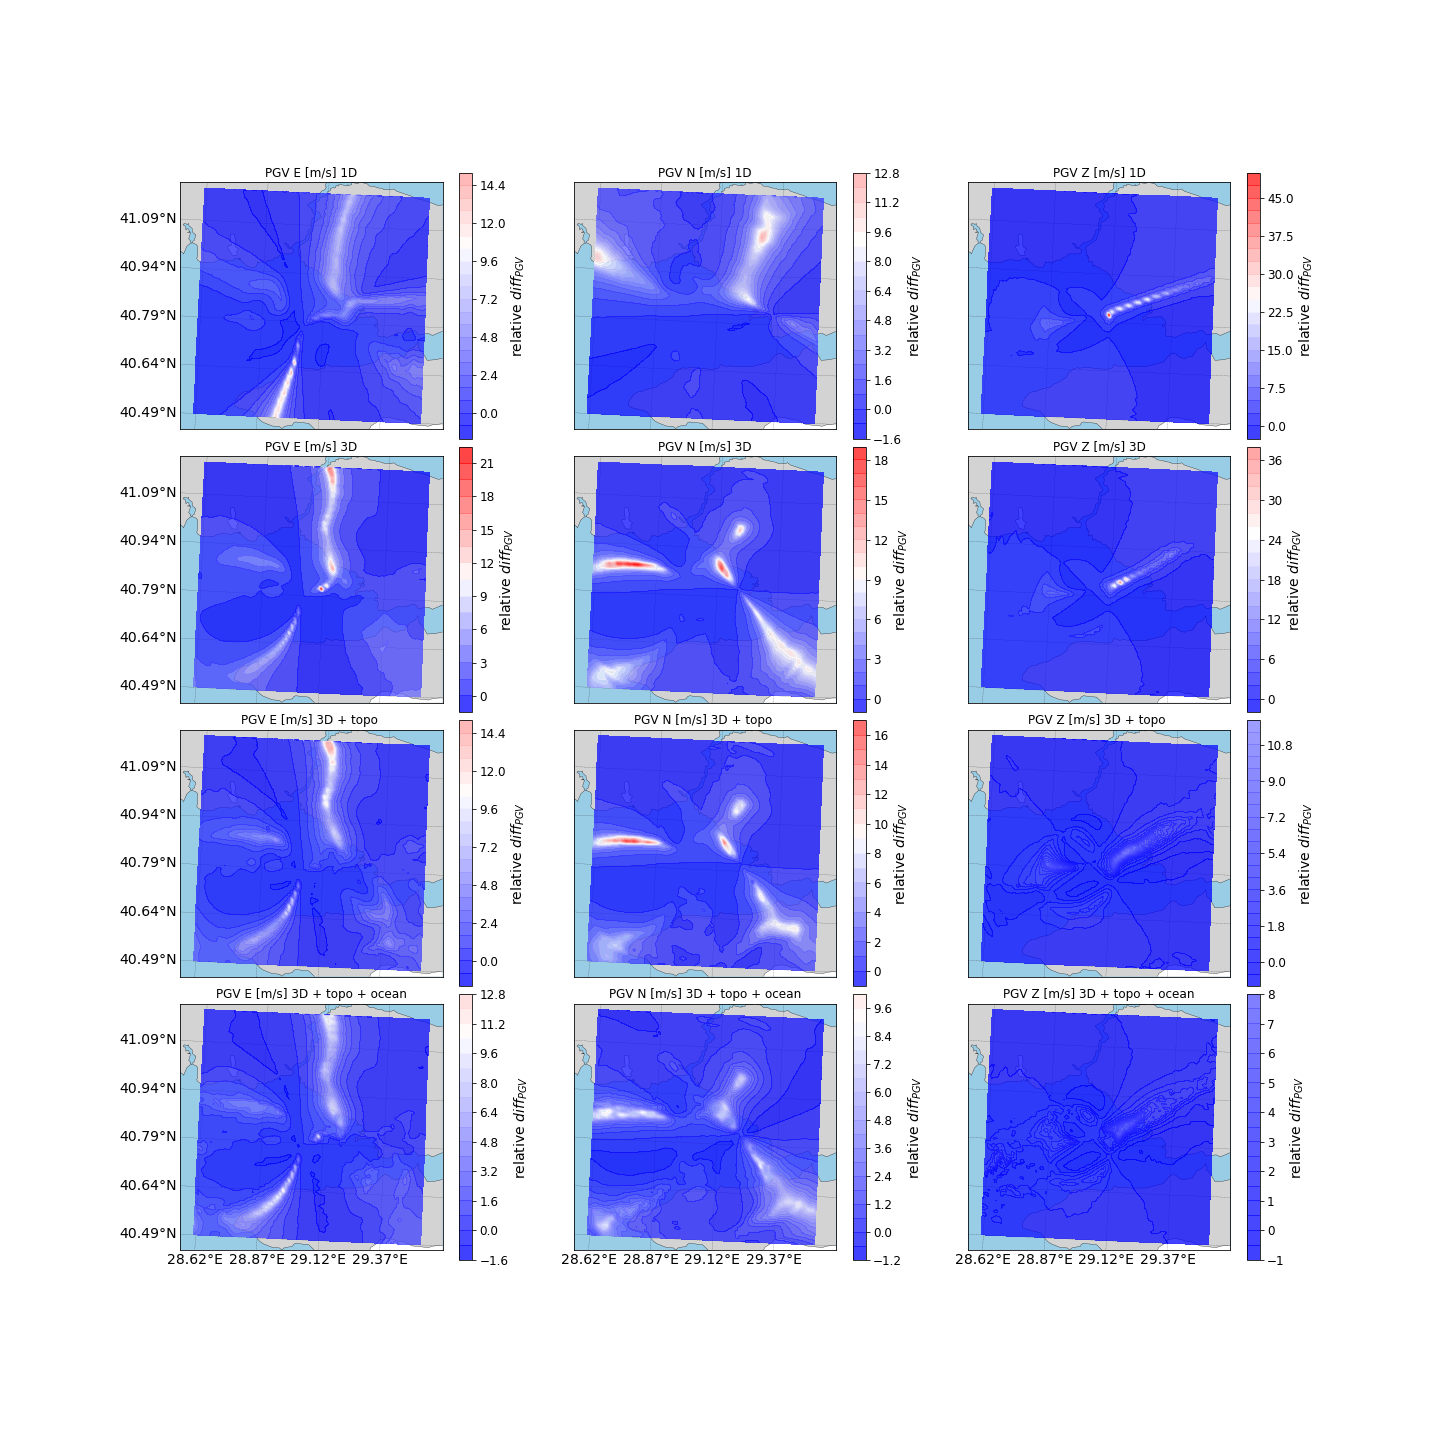
\includegraphics[width=1\linewidth,trim = 2cm 5cm 1cm 5cm, clip]{images_results/strike_variation_epsilon25_sc2.png}
    \caption{CMT2 relative difference between a scenario with a strike variation of 22.5$\degree$ with respect to the reference scenario. Colourbar set to the total minima and maxima of the 11.25$\degree$ and 22.5$\degree$ plots for comparison.}
    \label{fig:ref_eps25-2}
\end{figure}

\FloatBarrier

%%%%%%%%%%%%%%%%%%%%%%%%%%%%%%
\subsection{dip}

\subsubsection{CMT1}

\begin{figure}[htb!]
    \centering
    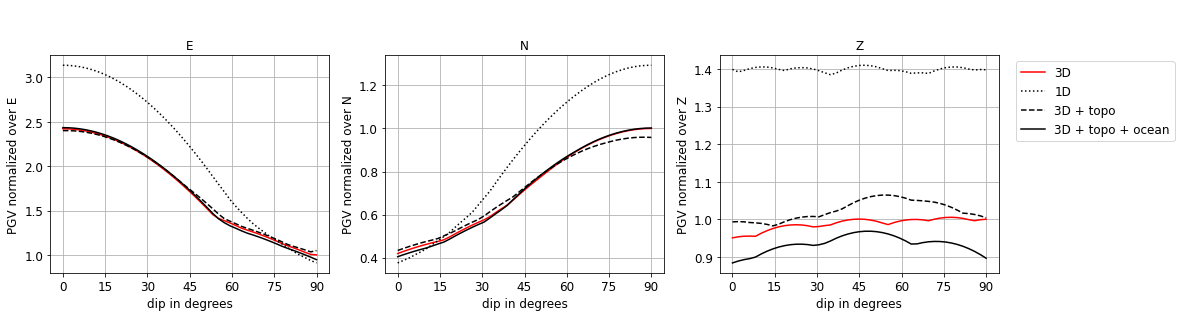
\includegraphics[width=.8\textwidth]{images_results/fullrange_dipvar_maxvals_sc1.png}
    \caption{Full 90$\degree$ range dip variation of the maximum measured PGV. Starting configuration CMT1: strike 90$\degree$, rake 180$\degree$}
    \label{fig:fullrange_1_dip}
\end{figure}

The dip ranges from 0-90$\degree$. The starting CMT1 has a purely vertical dip of 90$\degree$ and in this section the dip is varied between 45-90$\degree$. The coefficient of variation in Figure \ref{fig:ref_sigma1_dip} shows a very strong variation in the fault-normal directions, and little variability in the off-diagonal directions for the E and Z components. For both cases, this effect is strongly damped by including surface topography and ocean coupling. The variation of vertical movement is further damped inside the ocean coupling region of the domain. For the N component the oposite is true. The maximum values of variation reside in the off-diagonal directions of the fault, and these are amplified with the introduction of surface topography and the ocean. The lateral variations introduced by the 3D model have a stronger effect in the N direction compared to the E and Z directions. 

The maximum measured peak velocities for varying dip in Figure \ref{fig:fullrange_1_dip} show a very distinct pattern. As the vertical component stays relatively constant over the dip variation, the east and north components show an opposite trend. As the dip of the fault increases, the maximum velocities measured in the east direction decrease by a factor of 2.5 for the 3D, 3D + topo and 3D + topo + ocean simulations. This factor is higher for the 1D simulation. The north component shows a similar but opposite trend. The maximum velocity increases with increasing dip, in this case with a factor of 1.4. The Z component stays relatively stable, and is consistently over-estimated by the 1D model with respect to the other models. The 3D + topo + ocean model de-amplifies the maximum PGV by a factor of 0.9. This is consistent with the observations in the $\text{Cv}$ for the vertical diretion.

Considering the relative differences at 11.25$\degree$ and 22.5$\degree$ rotations of the dip in Figures \ref{fig:ref_eps12-1_dip} and \ref{fig:ref_eps25-1_dip}, we can observe a similar trend as in the variation of the strike angle. Variation of the dip in the E and Z directions has the most influence on the fault-normal PGVs. The strongest difference is observed in the E directions in the 3D and 1D flat models, where a distinct peak in relative difference is dominant at the source location. This peak is significantly de-amplified by the topography and ocean simulations. For the vertical Z direction, the peak velocity differences are concentrated along the fault strike. The N directions shows its peak variations to be significantly lower than the E and Z models. In this case, the peak velocity is amplified with increasing domain complexity. The same observation as for the strike could be made when comparing between the two relative difference plots with double the angle of dip variation: the peak velocities have increased with a factor of two for an decrease of the dip with a factor of two. 

\begin{figure}[htb]
    \centering
    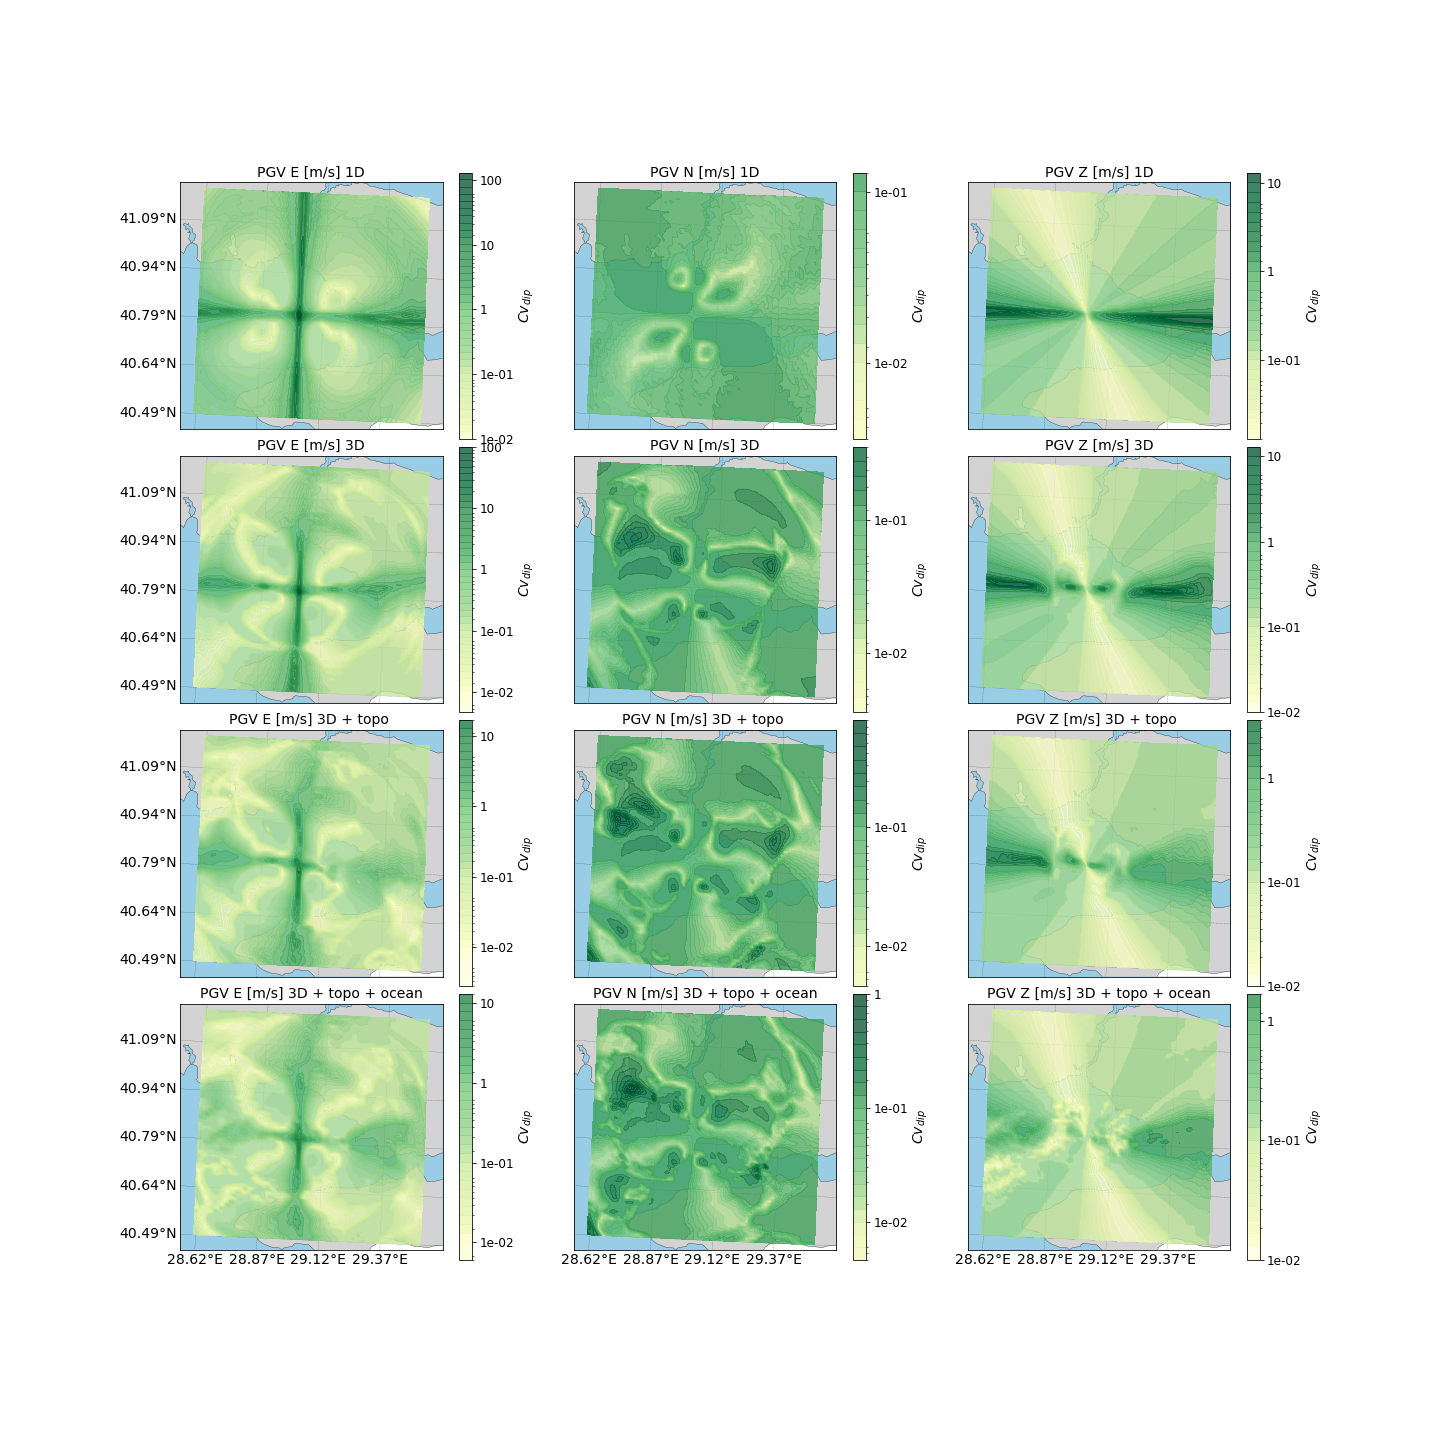
\includegraphics[width=1\linewidth,trim = 2cm 5cm 1cm 5cm, clip]{images_results/dip_variation_sigma_sc1.png}
    \caption{CMT1 coefficient of variation $Cv$ for dip, for each model domain in E, N and Z direction. Colourbar set to logarithmic to adequately show the large differences.}
    \label{fig:ref_sigma1_dip}
\end{figure}

\begin{figure}[h]
    \centering
    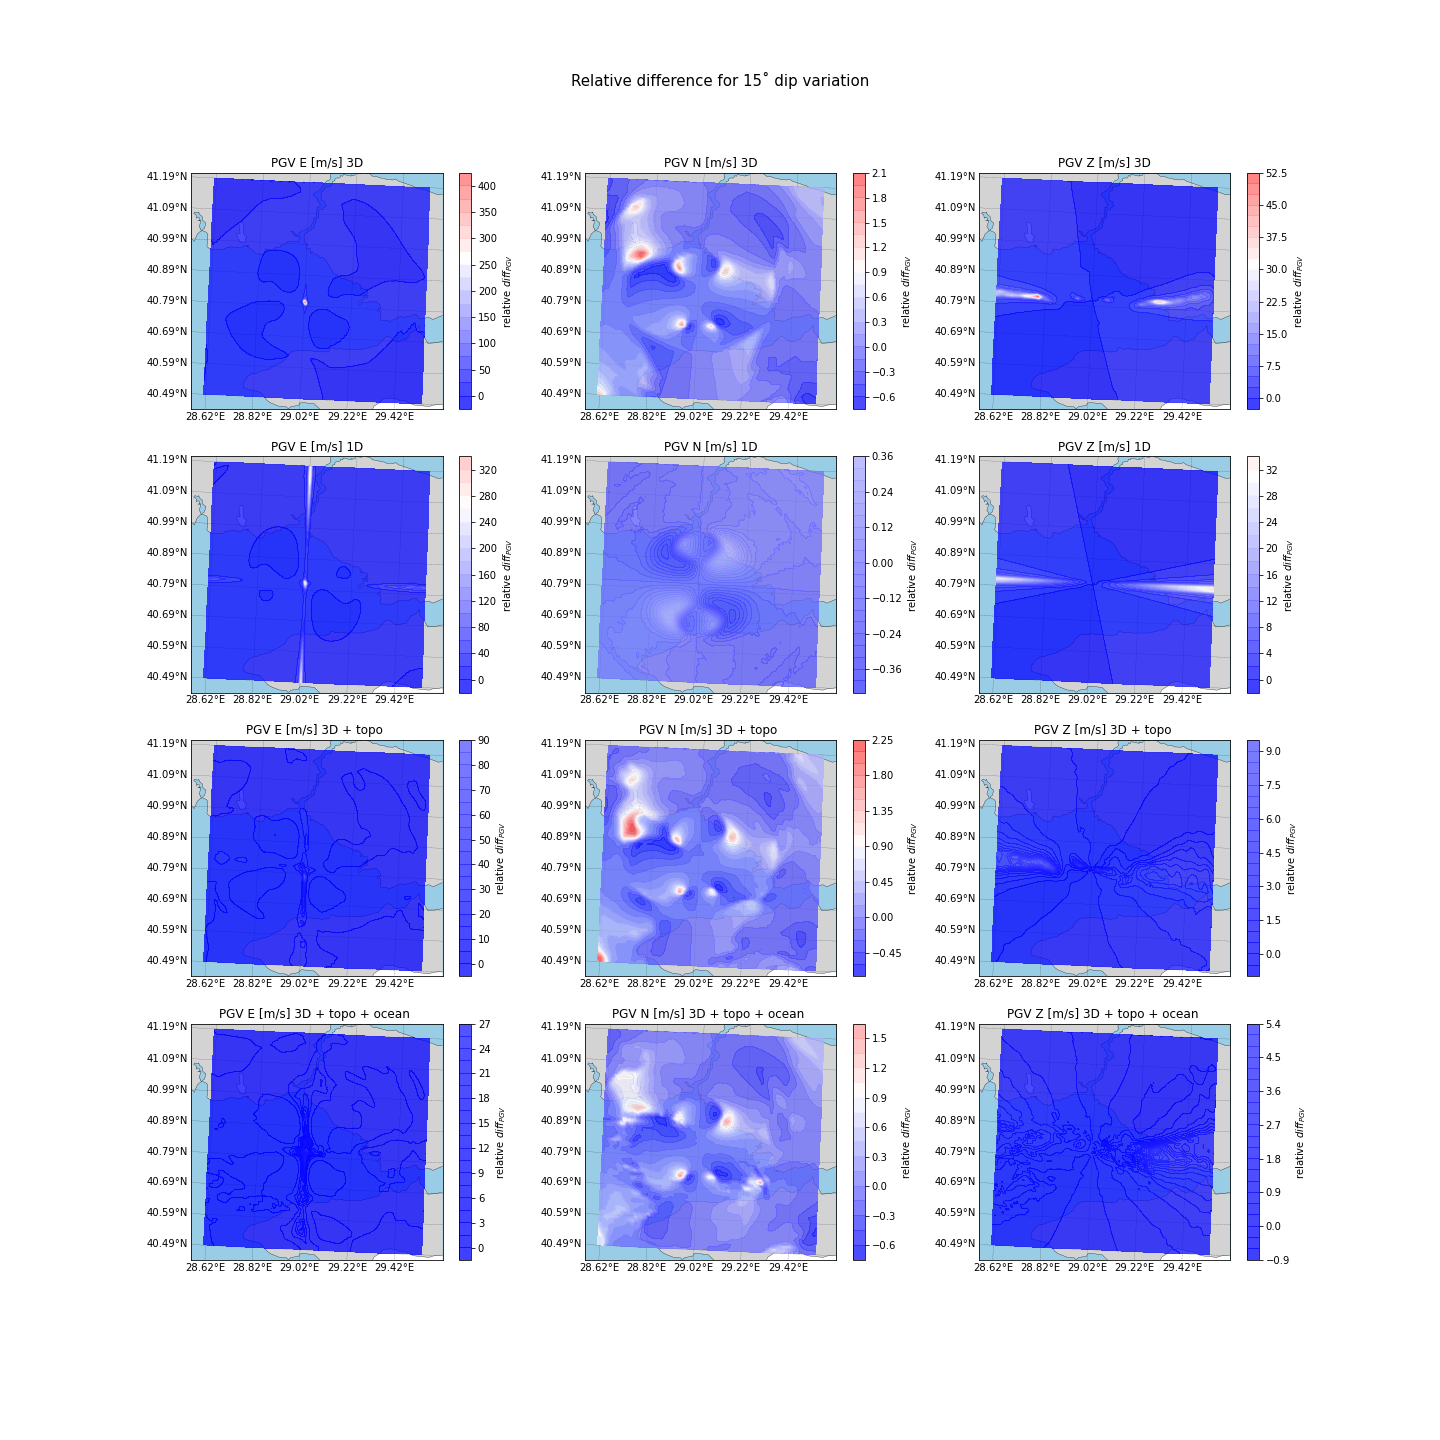
\includegraphics[width=1\linewidth,trim = 2cm 5cm 1cm 5cm, clip]{images_results/dip_variation_epsilon12_sc1.png}
    \caption{CMT1 relative difference between a scenario with a dip variation of 11.25$\degree$ with respect to the reference scenario. Colourbar set to the total minima and maxima of the 11.25$\degree$ and 22.5$\degree$ plots for comparison.}
    \label{fig:ref_eps12-1_dip}
\end{figure}

\begin{figure}[h]
    \centering
    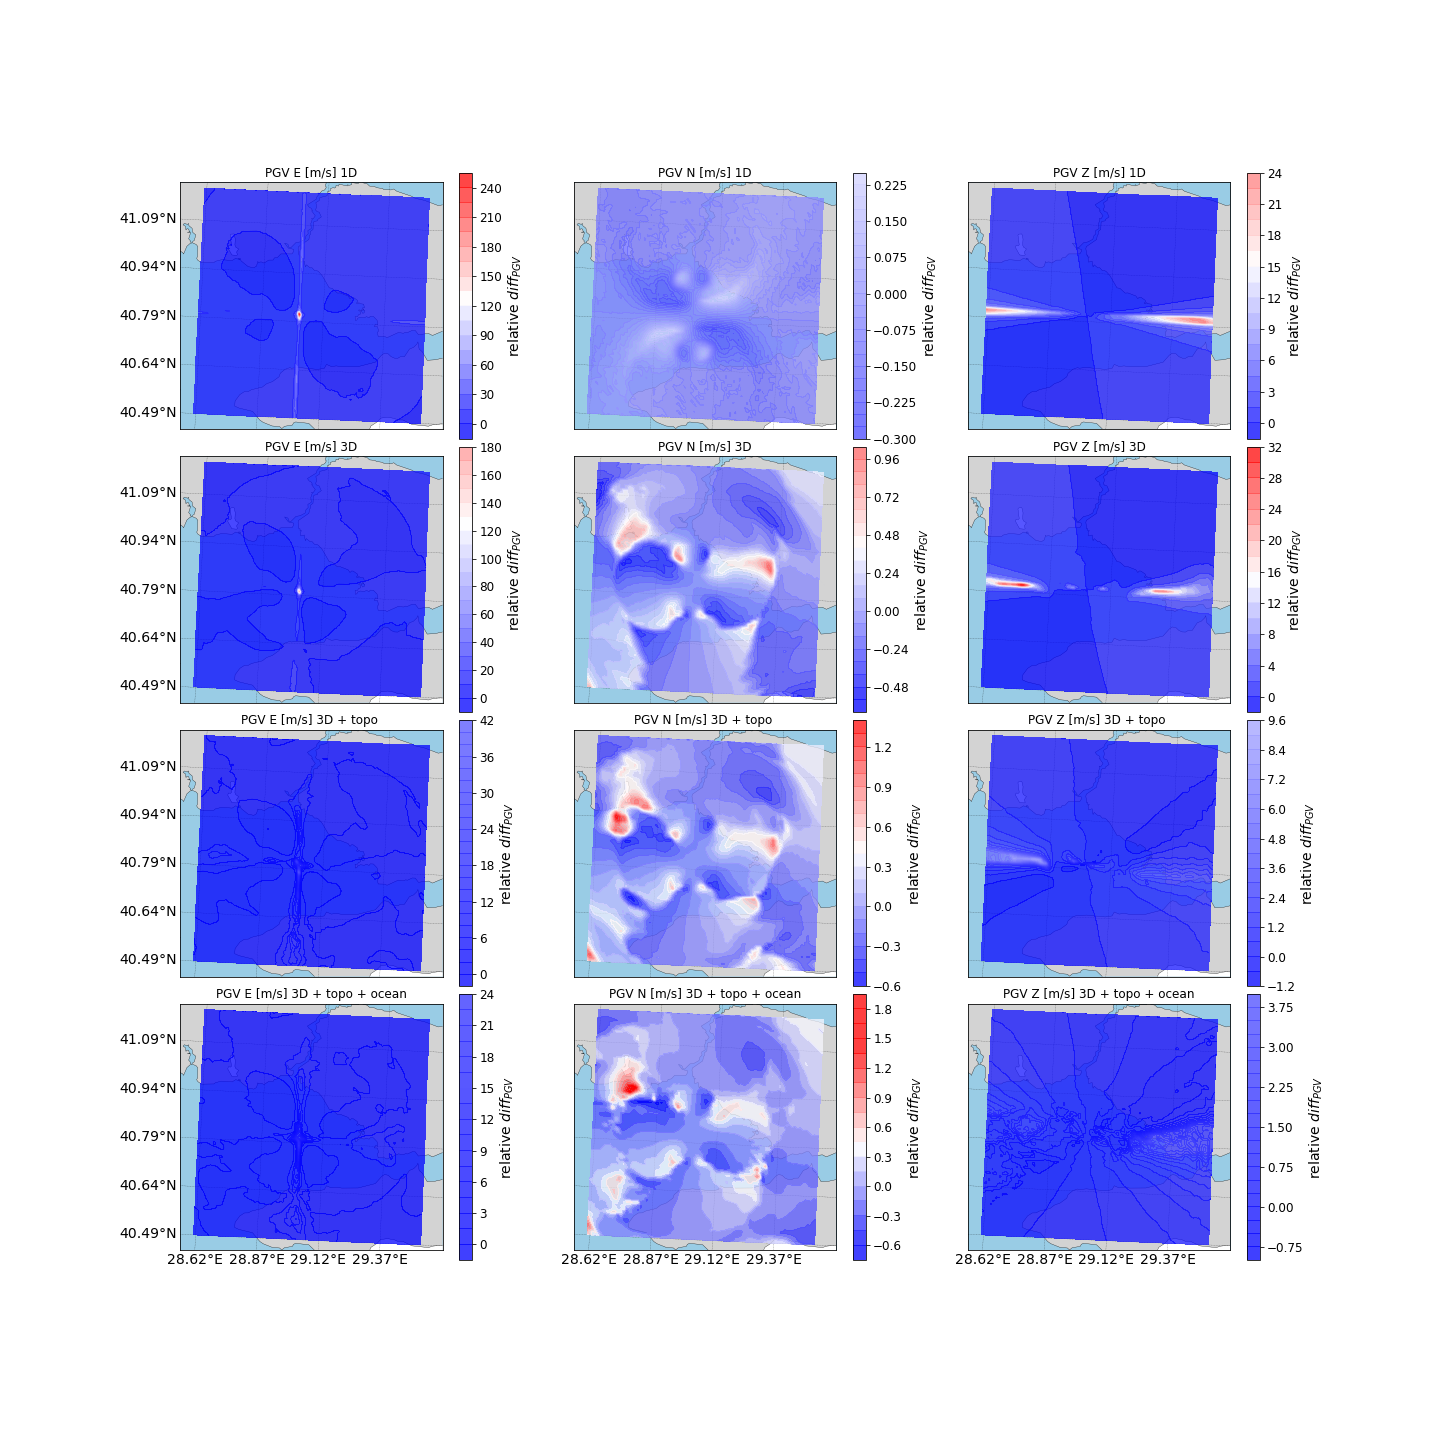
\includegraphics[width=1\linewidth,trim = 2cm 5cm 1cm 5cm, clip]{images_results/dip_variation_epsilon25_sc1.png}
    \caption{CMT1 relative difference between a scenario with a dip variation of 22.5$\degree$ with respect to the reference scenario. Colourbar set to the total minima and maxima of the 11.25$\degree$ and 22.5$\degree$ plots for comparison.}
    \label{fig:ref_eps25-1_dip}
\end{figure}

\FloatBarrier

\subsubsection{CMT 2}

\begin{figure}[htb!]
    \centering
    \subfloat[]{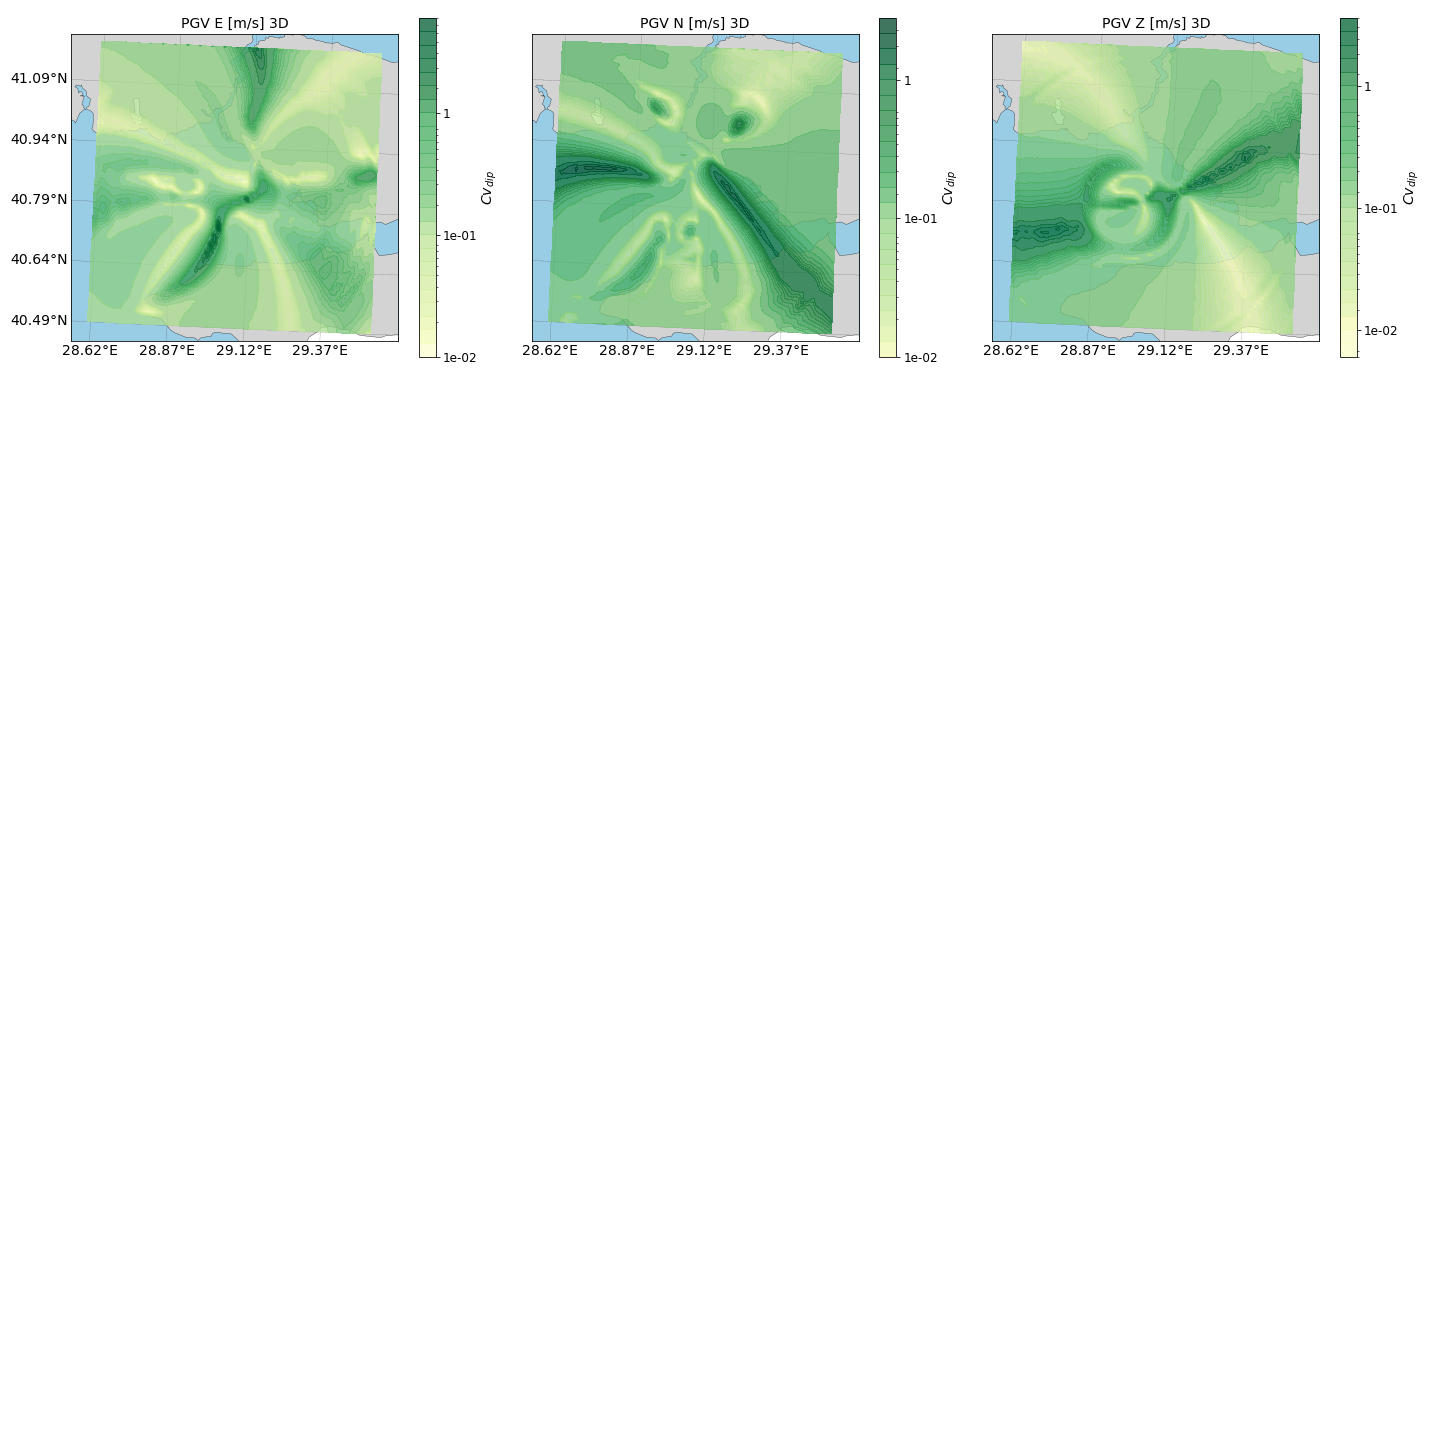
\includegraphics[width=15cm, trim= 0cm 38cm 0cm 0cm, clip ]{images_results/dip_variation_sigma_cut.png}}%
    \qquad
    \subfloat[]{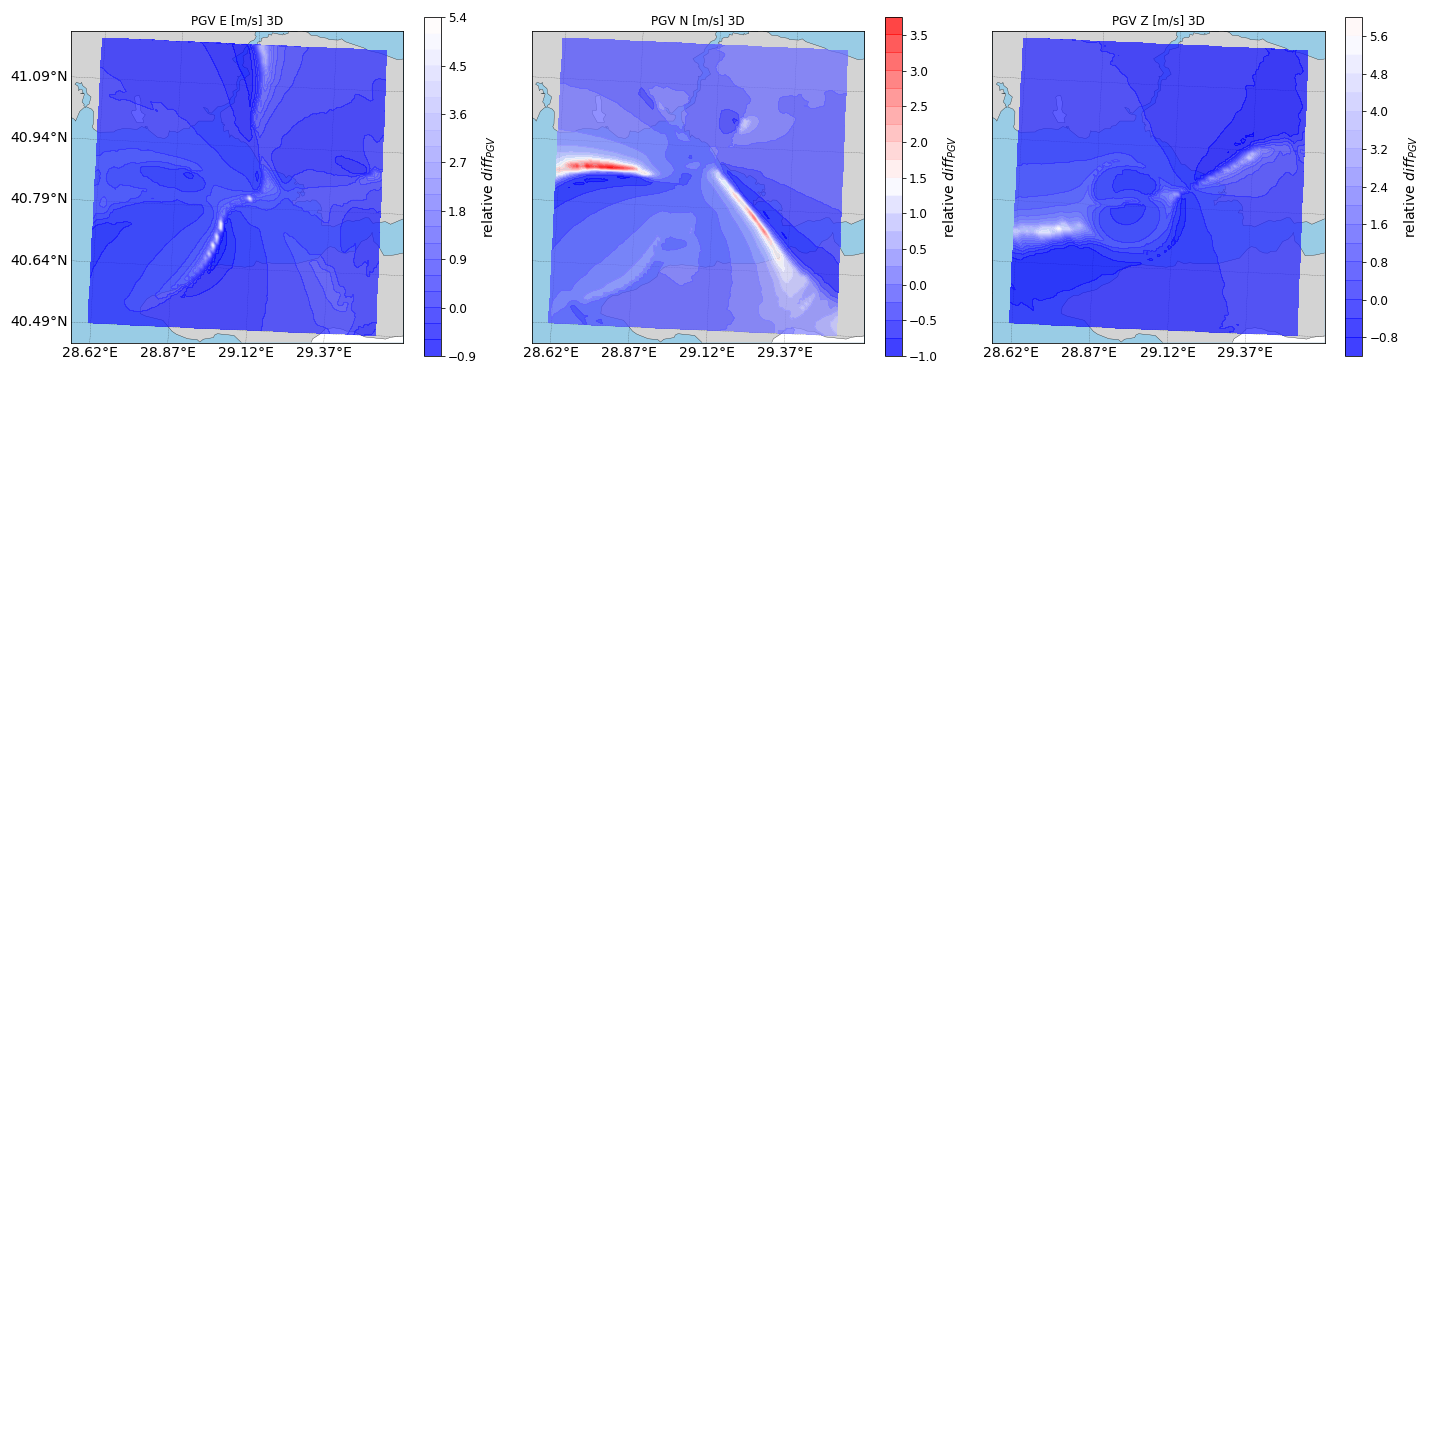
\includegraphics[width=15cm, trim= 0cm 38cm 0cm 0cm, clip ]{images_results/dip_variation_epsilon12_cut.png}}
    \qquad
    \subfloat[]{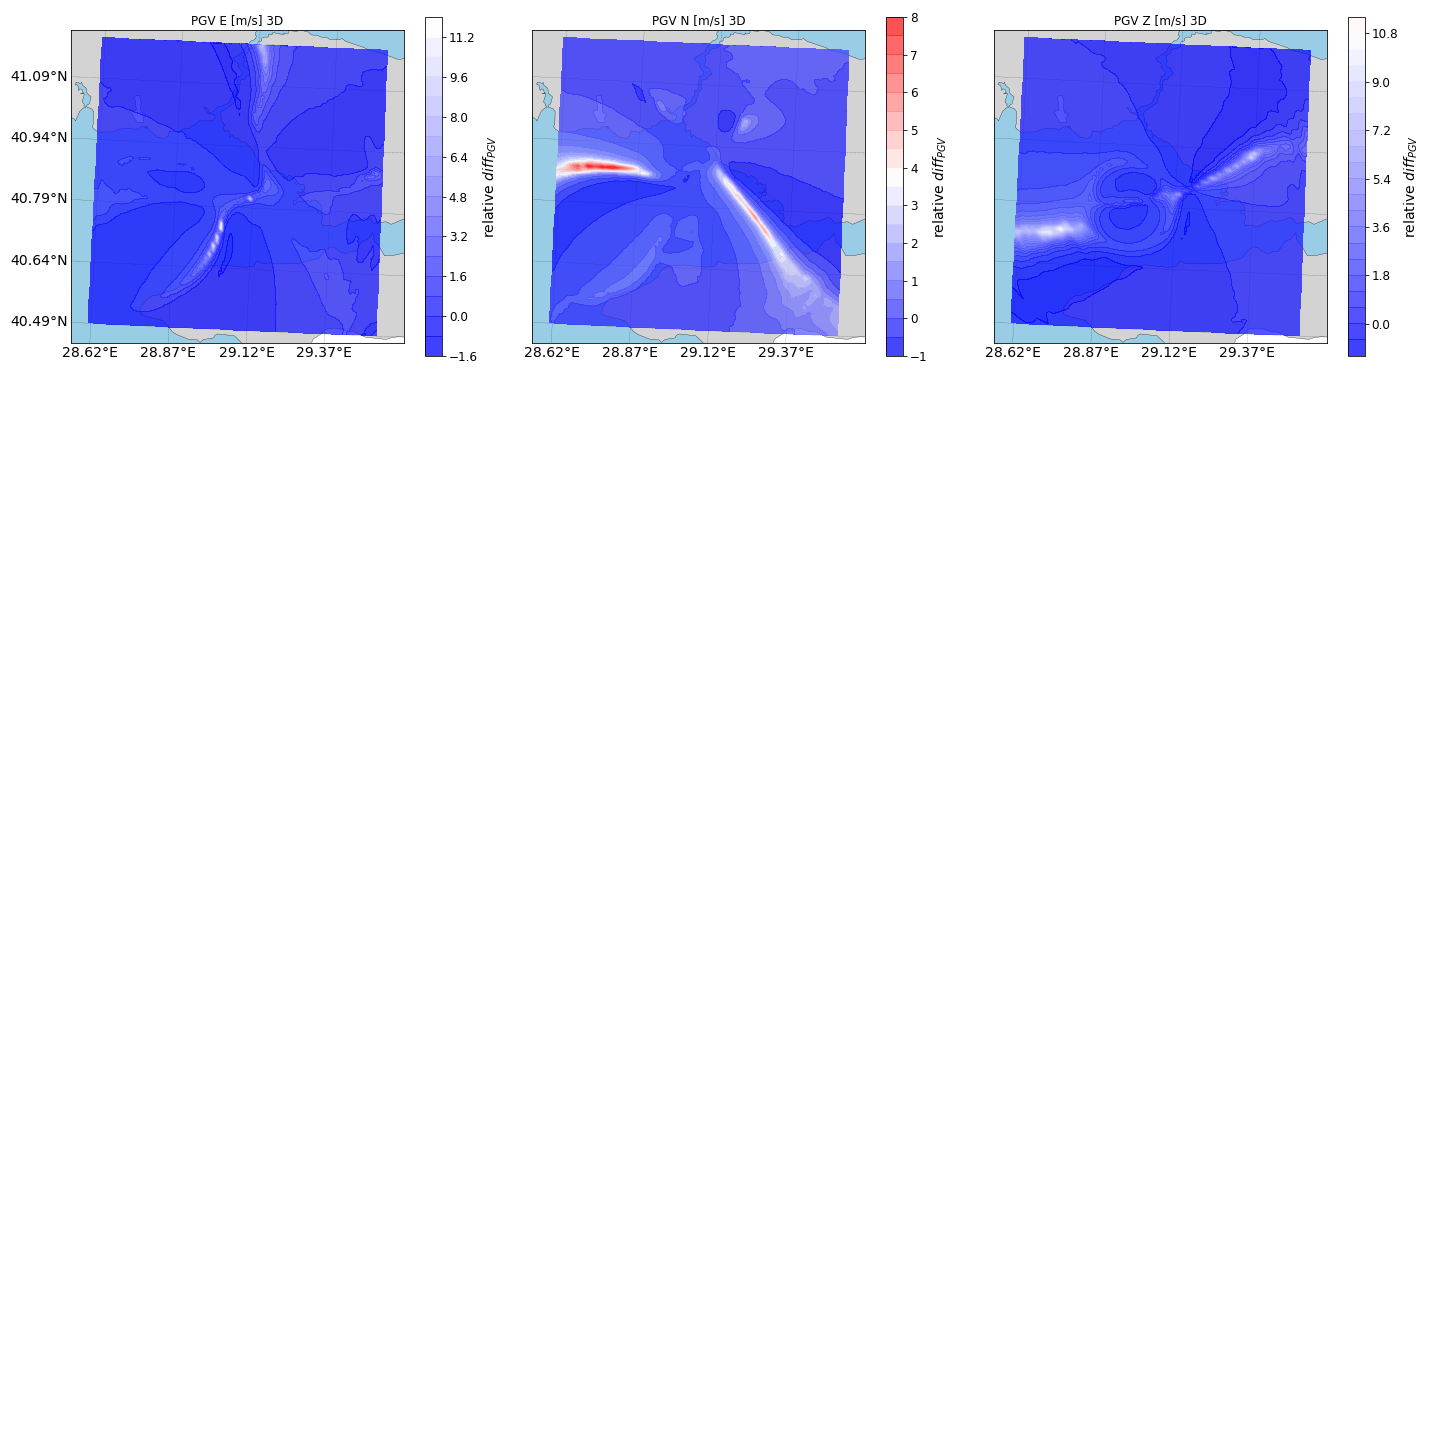
\includegraphics[width=15cm, trim= 0cm 38cm 0cm 0cm, clip ]{images_results/dip_variation_epsilon25_cut.png}}%
    \caption{}%
    \label{fig:dip_CMT2}%
\end{figure}



\FloatBarrier

\subsection{Rake}

\subsubsection{CMT1}

\begin{figure}[h!]
    \centering
    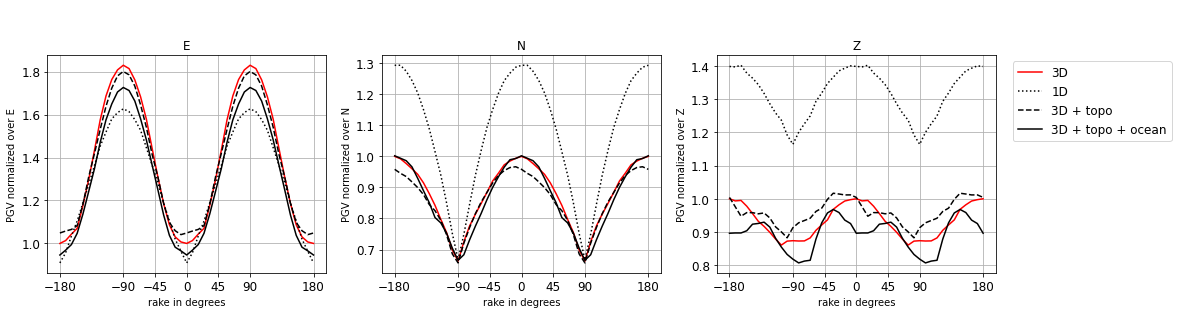
\includegraphics[width=0.8\textwidth]{images_results/fullrange_rakevar_maxvals_sc1.png}
    \caption{Full 90$\degree$ range rake variation of the maximum measured PGV. Starting configuration CMT1: strike 90$\degree$, dip 90$\degree$}
    \label{fig:fullrange_1_rake}
\end{figure}

The rake has a range between -180 to $+$180$\degree$, and is varied for 90$\degree$ both in the negative and positive directions. Figure \ref{fig:ref_sigma1_rake} shows the $\text{Cv}$ for these variations. On first glance, it becomes clear that the main variations in PGV take place in the E component in the fault-normal direction. The Z-direction differs from previous observations in $\text{Cv}$ for the strike and dip, as its main variations are now not only concentrated along the fault strike, but also along the off-diagonal directions as the rake deviation from 180$\degree$ introduces an oblique component to the faulting mechanism. This pattern is again symmetrical for the 1D scenario, and perturbations are introduced by the 3D model, topography and ocean implementation in the modelling domain. The 3D model introduces a stronger standard variation to the east and south of the fault strike. Further observations in the vertical direction are that the velocities along the fault strike are de-amplified by the ocean implementation, whereas this is not the case for the off-diagonal peak velocities. The north direction measures an increase of variation with increasing model domain complexity once again. Where the 1D model seems less sensitive to the variations of rake, the 3D model amplifies this effect by almost a factor of magnitude. Introduction of an ocean in the domain focuses the eastern peak variations towards the south-east. 

In Figures \ref{fig:ref_eps12-1_rake} and \ref{fig:ref_eps25-1_rake}, the rake is varied for -15$\degree$ and -30$\degree$ with respect to the 180$\degree$ starting point: more towards a normal fault configuration. The general observation of maximum PGV doubling with a variation twice as high also holds in this case. Here we see again that the fault-normal differences are de-amplified by the introduction of an ocean layer. 




\begin{figure}[htb]
    \centering
    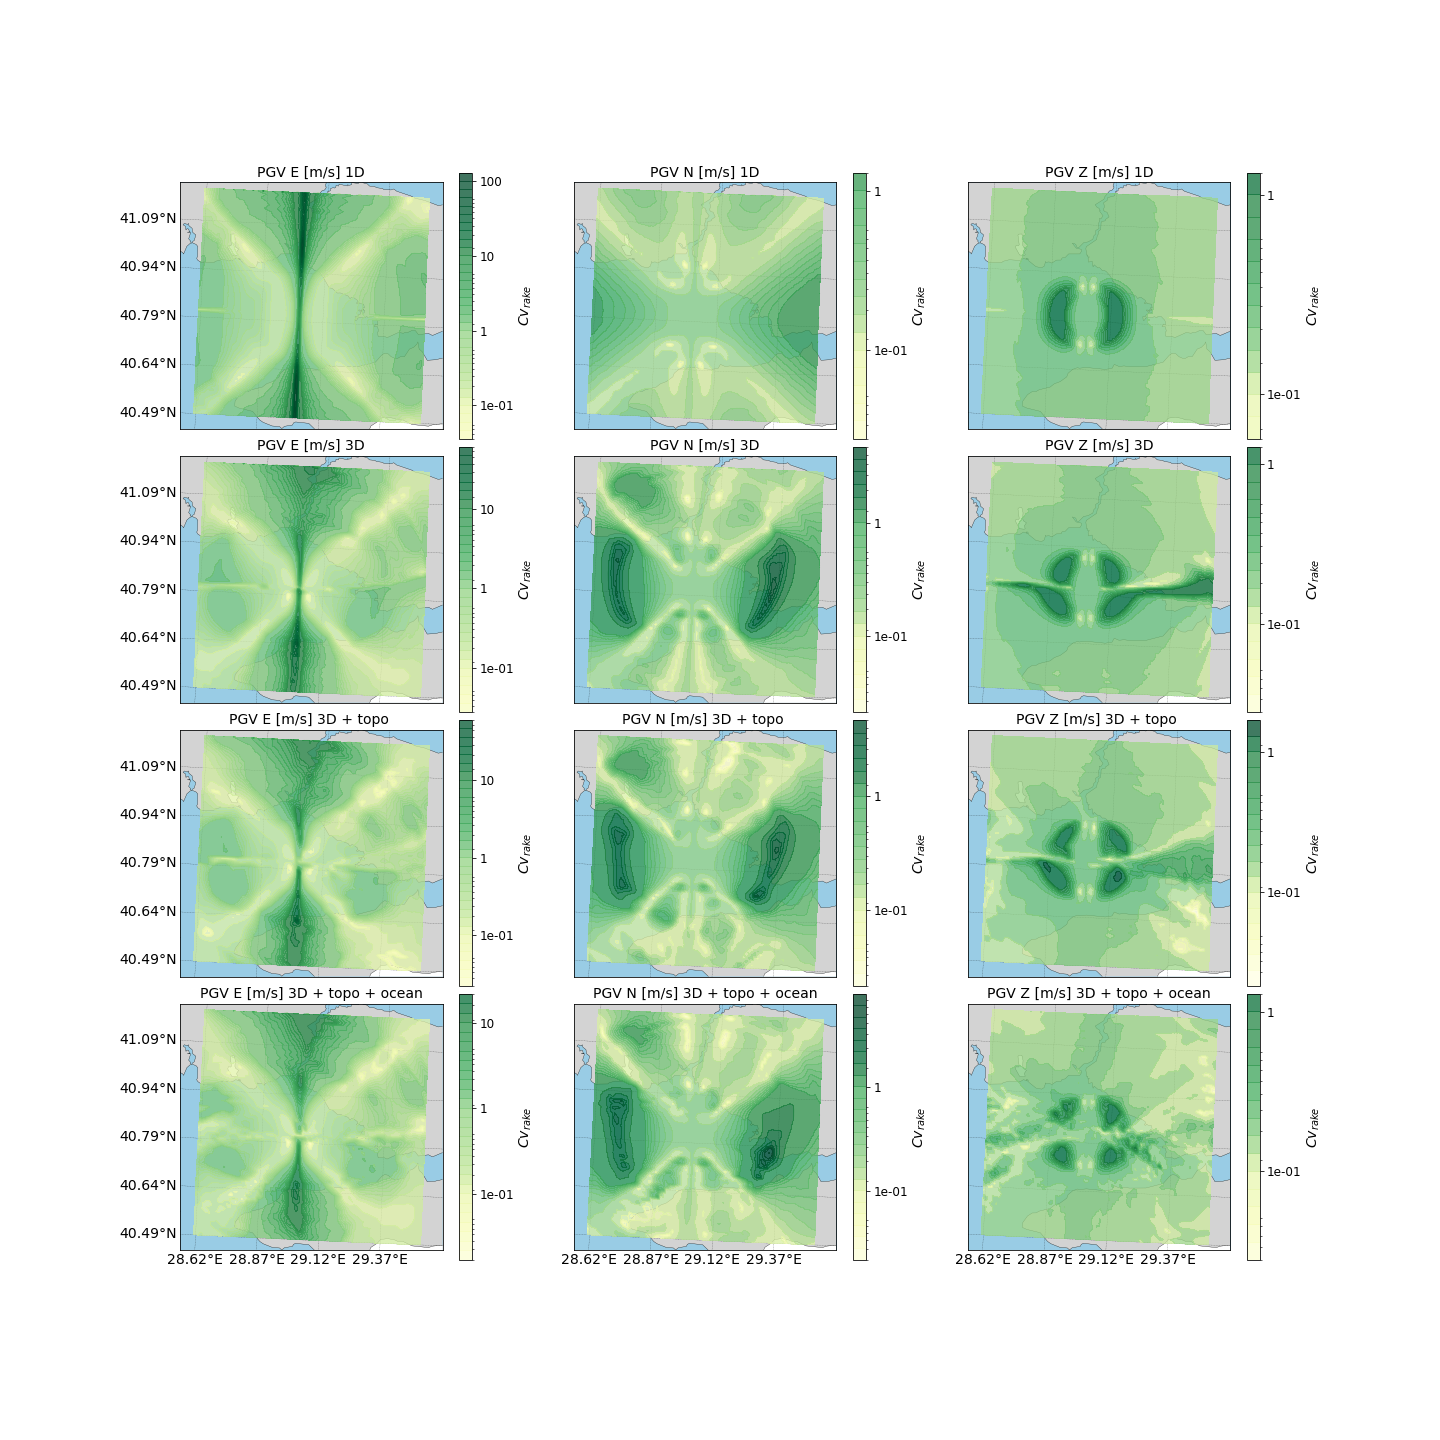
\includegraphics[width=1\linewidth,trim = 2cm 5cm 1cm 5cm, clip]{images_results/rake_variation_sigma_sc1.png}
    \caption{CMT1 coefficient of variation $Cv$ for rake, for each model domain in E, N and Z direction. Colourbar set to logarithmic to adequately show the large differences.}
    \label{fig:ref_sigma1_rake}
\end{figure}

\begin{figure}[h]
    \centering
    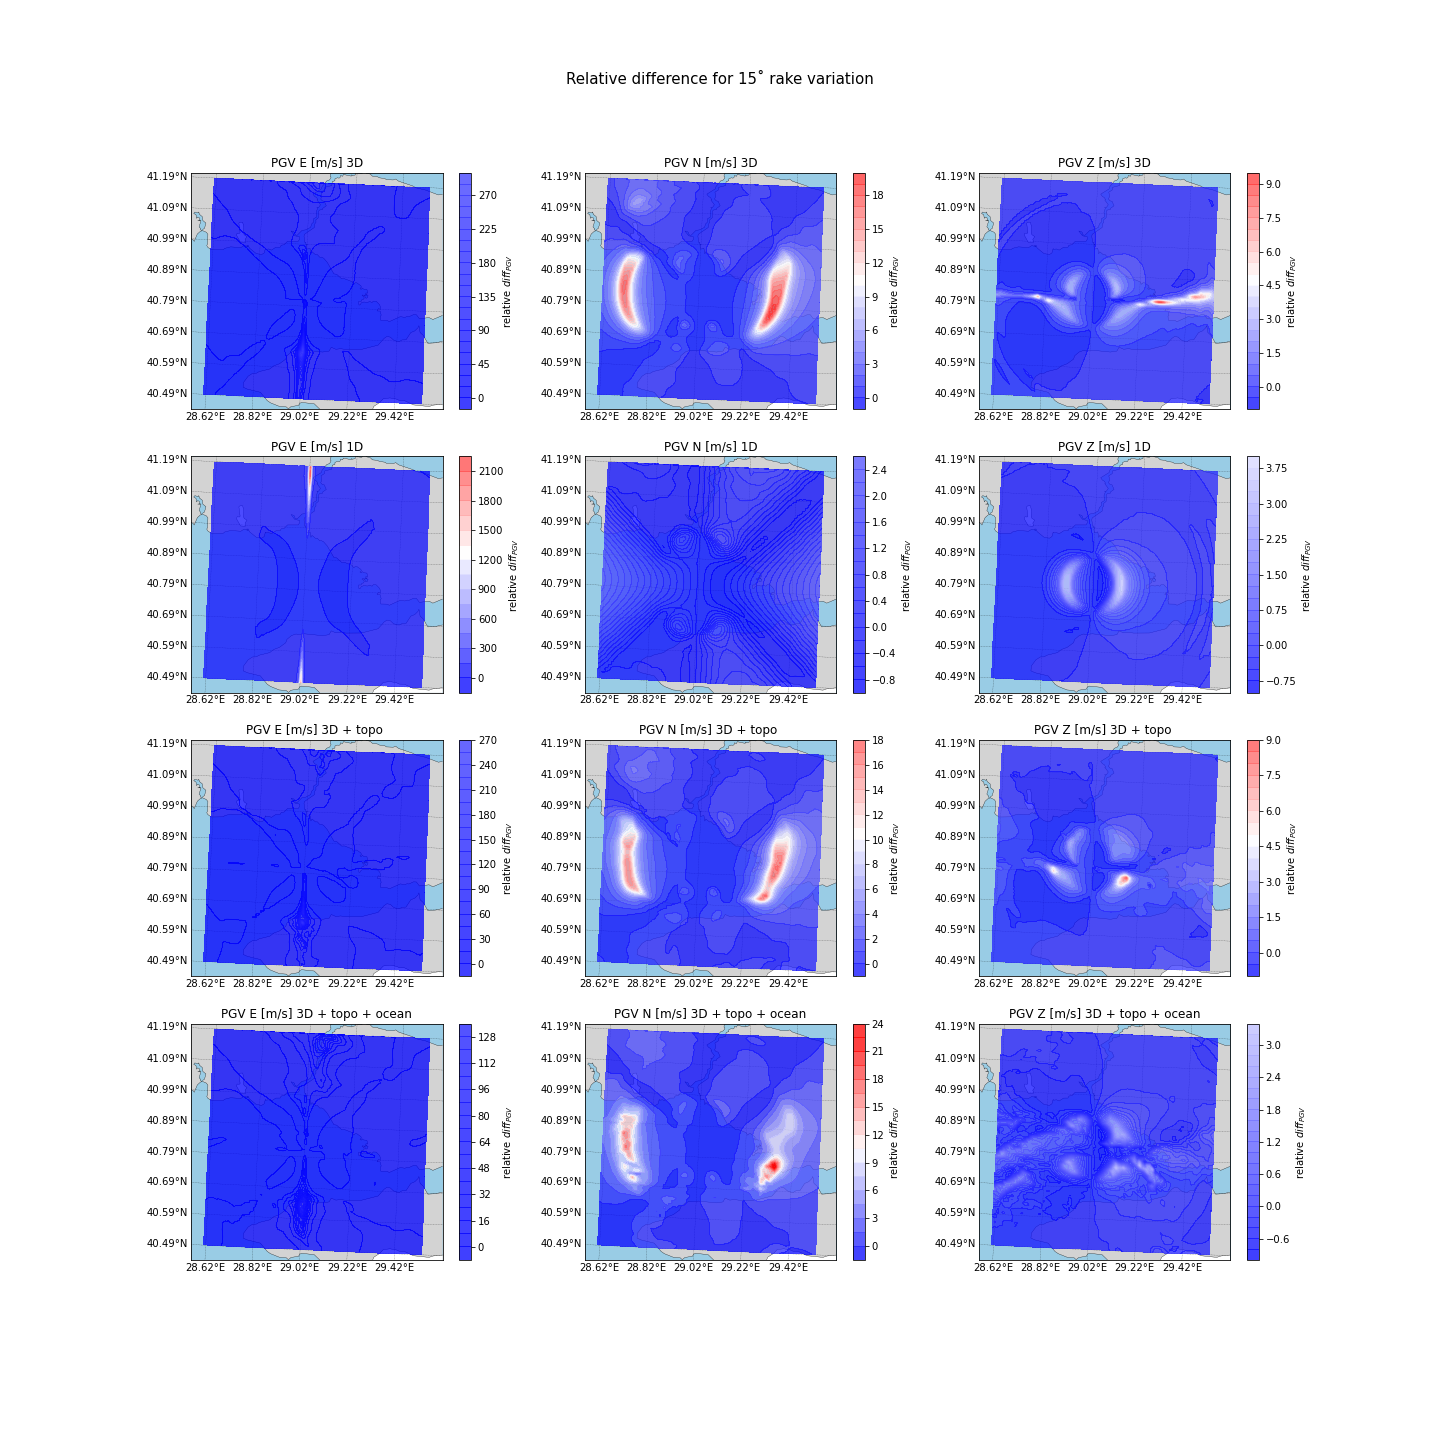
\includegraphics[width=1\linewidth,trim = 2cm 5cm 1cm 5cm, clip]{images_results/rake_variation_epsilon12_sc1.png}
    \caption{CMT1 relative difference between a scenario with a rake variation of 11.25$\degree$ with respect to the reference scenario. Colourbar set to the total minima and maxima of the 15$\degree$ and 30$\degree$ plots for comparison.}
    \label{fig:ref_eps12-1_rake}
\end{figure}

\begin{figure}[h]
    \centering
    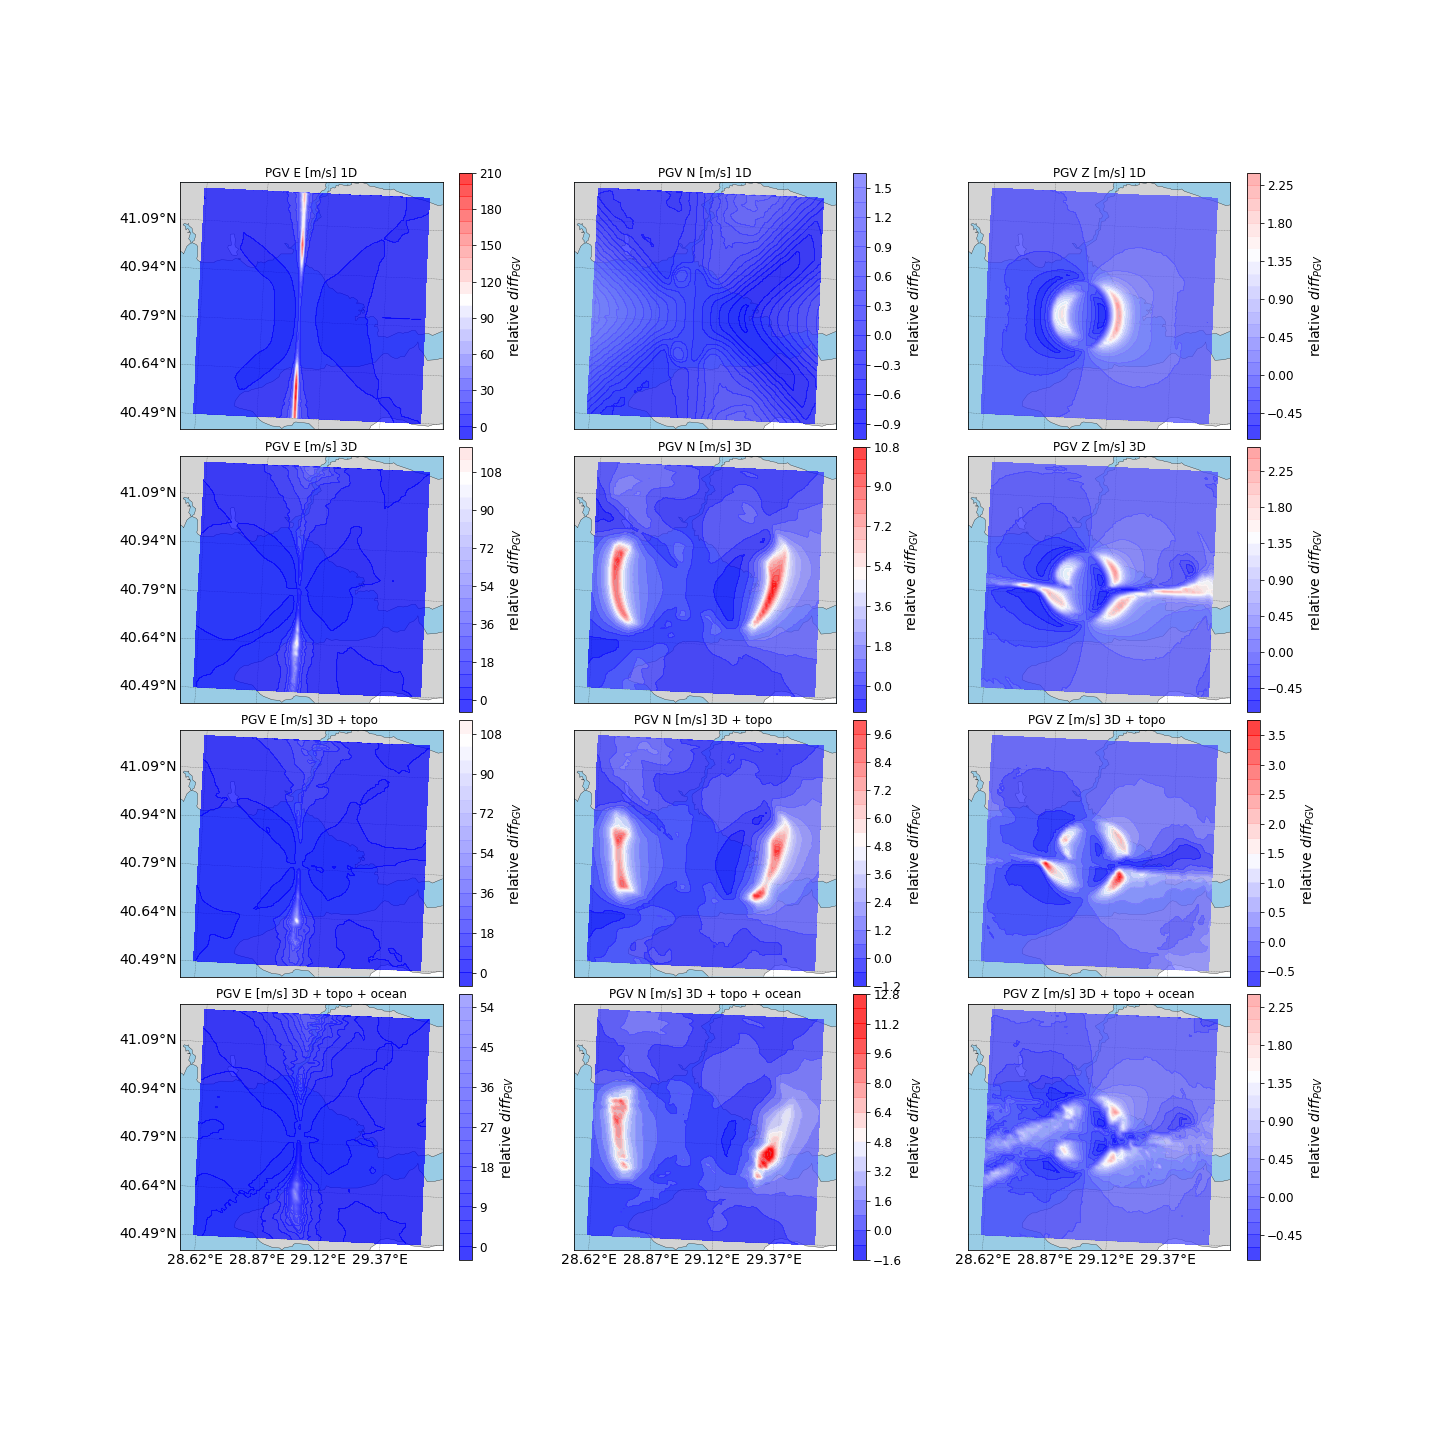
\includegraphics[width=1\linewidth,trim = 2cm 5cm 1cm 5cm, clip]{images_results/rake_variation_epsilon25_sc1.png}
    \caption{CMT1 relative difference between a scenario with a rake variation of 30$\degree$ with respect to the reference scenario. Colourbar set to the total minima and maxima of the 15$\degree$ and 30$\degree$ plots for comparison.}
    \label{fig:ref_eps25-1_rake}
\end{figure}

\subsubsection{CMT2}





\subsection{CMT3, CMT4: other configurations}

The normal and thrust scenarios in CMT3 and CMT4, respectively, are modelled to test whether the observations made in the previous sections hold for scenarios other than a strike-slip fault. 


\FloatBarrier


%%%%%%%%%%%%%%%%%%%%%%%%%%%%%%

\section{Source depth}

\hl{To do: show how shifting the location of the source mostly shifts the pattern with that amount meters at this scale. Show the variation of depth and its effects on PGV in the different domains}

\begin{figure}[ht!]
    \centering
    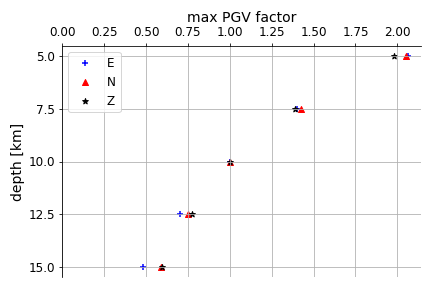
\includegraphics[width=.5\linewidth]{images_results/maxPGV_Depth.png}
    \caption{Caption}
    \label{fig:depth_maxpgv}
\end{figure}

\begin{figure}[h!]
    \centering
    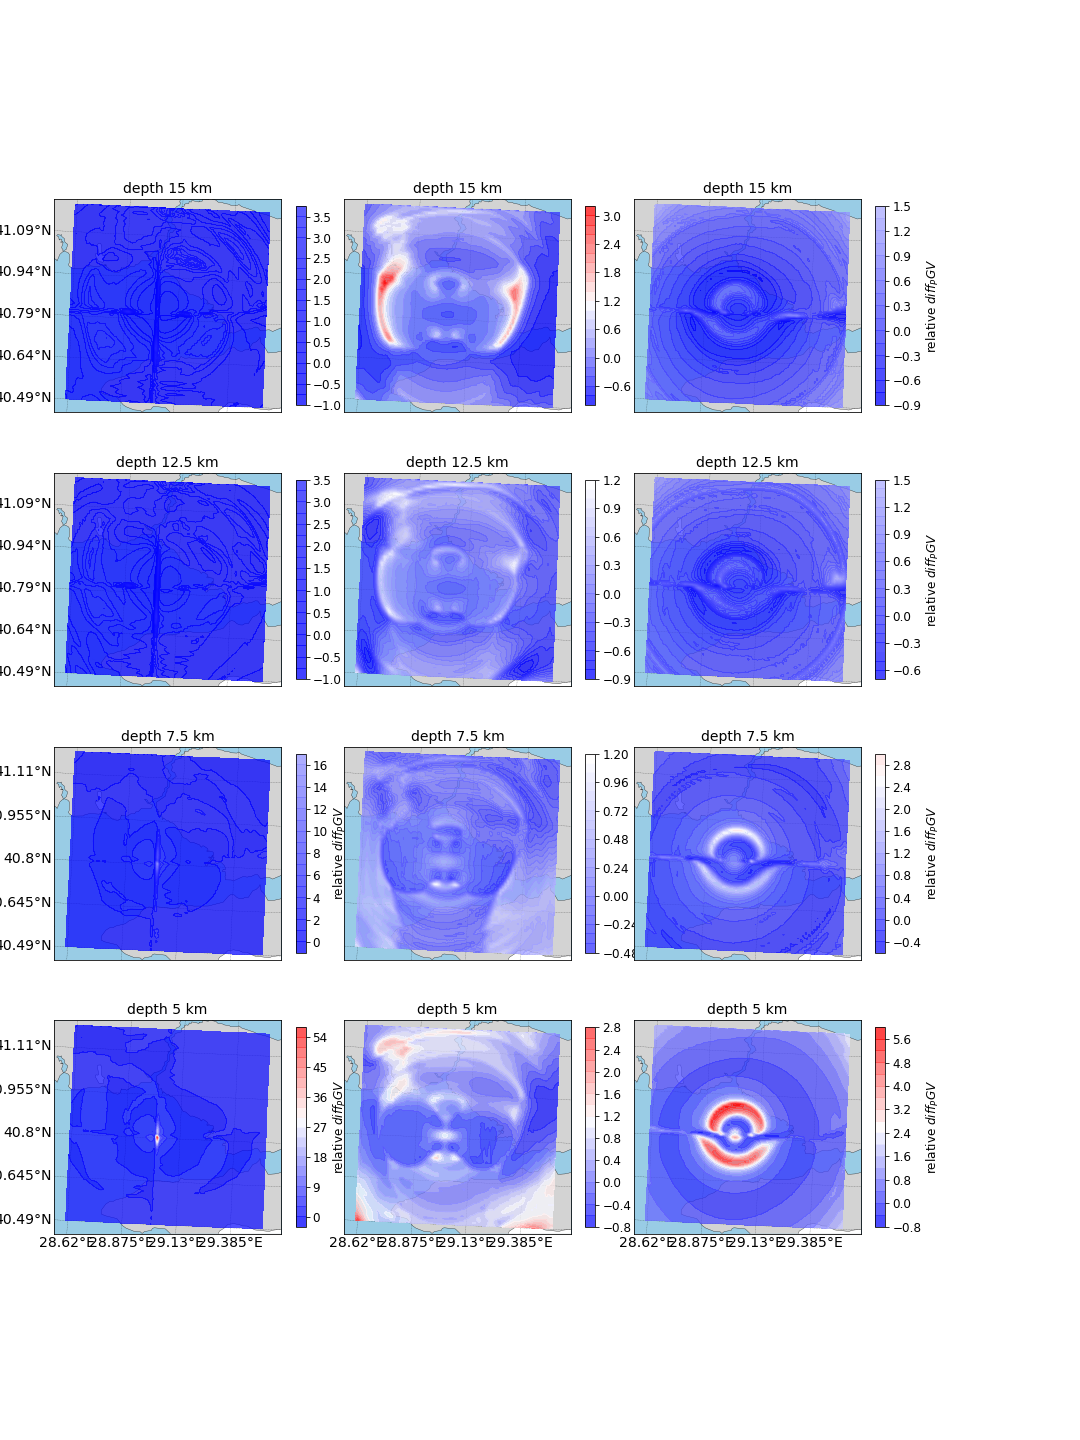
\includegraphics[width=1.0\linewidth, trim= 0cm 4cm 2cm 4cm, clip]{images_results/Ref_scenarios_normalized_depth.png}
    \caption{Relative difference between reference source depth of 10 km and sources at depths 15, 12.5, 7.5 and 5 km depth. All compositions are CMT1.}
    \label{fig:depth_diff}
\end{figure}

\FloatBarrier

\section{Short case study of a $M_w 7.0$ earthquake}

Although a CMT source representation is not an accurate approximation for earthquakes of $> Mw ??$, it is the type of source that can be inverted for directly after the event has occurred. As discussed earlier in section \hl{section}, it is the first step in the proposed urgent workflow of ChEESE  before a dynamic kinematic rupture scenario is simulated. To put the relative values of the previous sections into a practical perspective, we shortly assume a $M_w 7.0$ earthquake scenario at with the location, depth and nodal plane at CMT2. 

\hl{To do: Just to give some context to the relative cases of before, show a map with actual PGV values and the amount of standard deviation from this in the context of this scenario. Also show records at the three stations of this event.}

%[image 1D E, N, Z real values PGV, PGA , Arias]

%[image 3D E, N, Z real values + difference to 1D PGV, Arias]

%[image 3D + topo E, N, Z real values + difference to 3D PGV, Arias]

%[image 3D + topo  \& Ocean E, N, Z real values + difference to 3D + topo PGV, Arias]

%[image Spectral response on 3 real station locations]

\begin{itemize}
    \item comment on changes in pattern of the real values 
    \item comment on ground shaking of this scenario
\end{itemize}








\end{document}